%%%%%%%%%%%%%%%%%%%%%%%%%%%%%
%% Styles, packages and new commands
\input{../../Main/ML_Main.tex}
%%%%%%%%%%%%%%%%%%%%%%%%%%%%%
%% Edit the title page
\title{Machine Learning}
\subtitle{Module 3.2 - Models: Classification And Regression Trees}
\author[MOB]{Marc-Olivier Boldi}
\institute[HEC MSc Mgt BA]{Master in Management, Business Analytics, HEC UNIL}
\date{Spring 2025}
%%%%%%%%%%%%%%%%%%%%%%%%%%%%%
%%%%%%%%%%%%%%%%%%%%%%%%%%%%%
%%%%%%%%%%%%%%%%%%%%%%%%%%%%%
%%%%%%%%%%%%%%%%%%%%%%%%%%%%%
\begin{document}
%%%%%%%%%%%%%%%%%%%%%%%%%%%%%
\begin{frame}
  \titlepage
\end{frame}
%%%%%%%%%%%%%%%%%%%%%%%%%%%%%
\begin{frame}
\frametitle{Table of Contents}
	\tableofcontents
\end{frame}
%%%%%%%%%%%%%%%%%%%%%%%%%%%%%
%%%%%%%%%%%%%%%%%%%%%%%%%%%%%
\section{Concept}
%%%%%%%%%%%%%%%%%%%%%%%%%%%%%
%%%%%%%%%%%%%%%%%%%%%%%%%%%%%
\begin{frame}
\frametitle{CART}
CART stands for {\bf C}lassification {\bf A}nd {\bf R}egression {\bf T}rees. It consists of 
\begin{itemize}
\item A hierarchical set of binary rules,
\item A representation in a shape of a tree.
\end{itemize}
It applies to both regression and classification tasks.
\end{frame}
%%%%%%%%%%%%%%%%%%%%%%%%%%%%%
\begin{frame}
\frametitle{The prediction formula}
Iris data (on 105 data; 35/35/35).
\begin{columns}
\begin{column}{0.5\textwidth}
\begin{center}
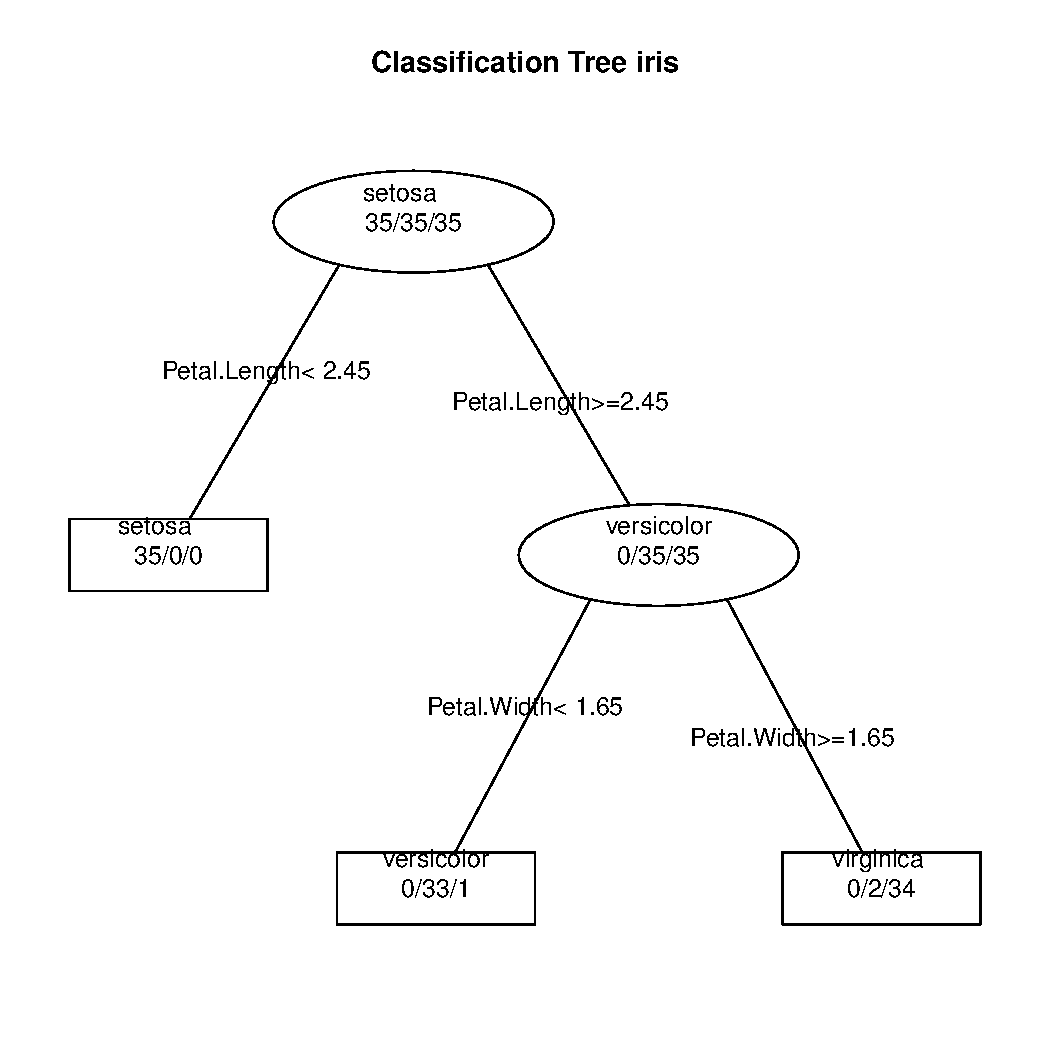
\includegraphics[width=6.5cm]{../../Graphs/IRIS_CART.pdf}
\end{center}
\end{column}
\begin{column}{0.5\textwidth}
\small
If Petal length $< 2.45$ then Setosa, else
\begin{itemize}
\item if Petal width $< 1.65$ then Versicolor, else Virginica.
\end{itemize}
\end{column}
\end{columns}
\end{frame}
%%%%%%%%%%%%%%%%%%%%%%%%%%%%%
\begin{frame}
\frametitle{The prediction formula}
The set of rules including the order of the features and the thresholds at each node can be embedded into a set of parameters $\theta$. \\
\vspace{0.3cm}
After the training, the tree contains of final nodes. We use the notation below,
\begin{itemize}
\item Applying the rules to features $x$ send the instance $(y,x)$ to the final node that we call $N(x)$.
\item In the training set $(y_1,x_1), \ldots, (y_n,x_n)$, the set of instances that were sent to node $N$ is called $I(N)$. E.g., $I(N)=\{1,3,4\}$ means that instances $(y_1,x_1),(y_3,x_3),(y_4,x_4)$ were sent to node $N$.
\item The prediction for features $x$ is noted $f(x;\theta)$. That prediction only depends on the node to which $x$ is sent. In other words,
$$
N(x) = N(x') \quad \Longrightarrow \quad f(x;\theta) = f(x';\theta).
$$ 
\end{itemize}
\end{frame}
%%%%%%%%%%%%%%%%%%%%%%%%%%%%%
\begin{frame}
\frametitle{The prediction formula: regression}
For regression, $f(x;\theta)$, the prediction for $x$, is the mean of the $y_i$'s that were sent to the node of $x$ during the training.\\
\vspace{0.3cm}
In more fancy terms, 
$$
f(x;\theta) = \frac{1}{|I(N(x))|}\sum_{i \in I(N(x))} y_i.
$$
\end{frame}
%%%%%%%%%%%%%%%%%%%%%%%%%%%%%
\begin{frame}
\frametitle{The prediction formula: classification}
For classification, 
\begin{itemize}
\item The node $N(x)$ has a predicted probability vector: probabilities one each possible class 
$$
p(x;\theta) = (p_1(x;\theta), \ldots, p_C(x;\theta)),
$$
\item The prediction $f(x;\theta)$ is the class that has highest probability:
$$
f(x;\theta) = \arg\max_{c=1,\ldots,C} p_c(x;\theta).
$$ 
\end{itemize}
The predicted probabilities $p(x;\theta)$ at node $N(x)$ are the proportions of each class taken on all the instances sent to $N(x)$ during the training.\\
\vspace{0.2cm}
In more fancy terms, for any class $c$,
$$
p_c(x;\theta) = \frac{1}{|I(N(x))|}\sum_{i \in I(N(x))} 1_{\{y_i = c\}}.
$$
\end{frame}
%%%%%%%%%%%%%%%%%%%%%%%%%%%%%
\begin{frame}
\frametitle{The loss function: regression}
For the regression case, the most used loss function is the MSE:
$$
\bar{\cal L}(\theta) = \frac{1}{n} \sum_{i=1}^n \left\{y_i - f(x_i;\theta)\right\}^2
$$
\end{frame}
%%%%%%%%%%%%%%%%%%%%%%%%%%%%%
\begin{frame}
\frametitle{The loss function: classification}
For the classification case, the most used loss is the {\bf entropy}. It is different from the one of logistic regression\footnote{For logistic regression, it is the cross-entropy.}. In the case of $C$ classes, the entropy is
\begin{eqnarray*}
{\cal L}(y, p) &=& - p_1 \log p_1 - p_2 \log p_2 - \cdots - p_C \log p_C\\
&=& - \sum_{c=1}^C p_C \log p_c.
\end{eqnarray*}
A the global entropy is thus
\begin{eqnarray*}
\bar{\cal L}(\theta) &=& - \sum_{i=1}^n\sum_{c=1}^C p_c(x_i;\theta) \log p_c(x_i;\theta).
\end{eqnarray*}
\end{frame}
%%%%%%%%%%%%%%%%%%%%%%%%%%%%%
\begin{frame}
\frametitle{The loss function: classification}
Other possible choices for the loss function are: \\
\vspace{0.3cm}
The {\bf classification error}: 
$$
{\cal L}(y,p) = 1 - p_y.
$$
If $y=c$, then $p_c$ should be large and $1-p_c$ should be small.\\
\vspace{0.3cm}
The {\bf Gini index}:
$$
{\cal L}(y,p) = p_1(1-p_1) + \cdots + p_C(1-p_C) = \sum_{c=1}^C p_c(1-p_c).
$$
This index is smaller if $p$ has one large component and the other ones small (e.g., $(1,0,0,0)$). It is thus minimum when the prediction is certain. For this, it is similar to the entropy.
\end{frame}
%%%%%%%%%%%%%%%%%%%%%%%%%%%%%
\begin{frame}
\frametitle{The greedy algorithm}
Finding the optimal $\theta$ cannot be obtained using a Newton-Raphson algorithm because $f(x;\theta)$ is not differentiable.\\ 
\vspace{0.3cm}
To obtain the optimal $\hat{\theta}$, one should search among all possible splitting combinations. The complexity of such task is enormous and cannot be achieved even with the most powerful imaginable computers. \\
\vspace{0.3cm}
An approximate solution is obtained by the {\bf greedy algorithm}.
\end{frame}
%%%%%%%%%%%%%%%%%%%%%%%%%%%%%
\section{The greedy algorithm}
%%%%%%%%%%%%%%%%%%%%%%%%%%%%%
\begin{frame}
\frametitle{Splitting the data space}
The tree splits the space into rectangles\footnote{Several trees may be equivalent.}. Below with two features:
\begin{center}
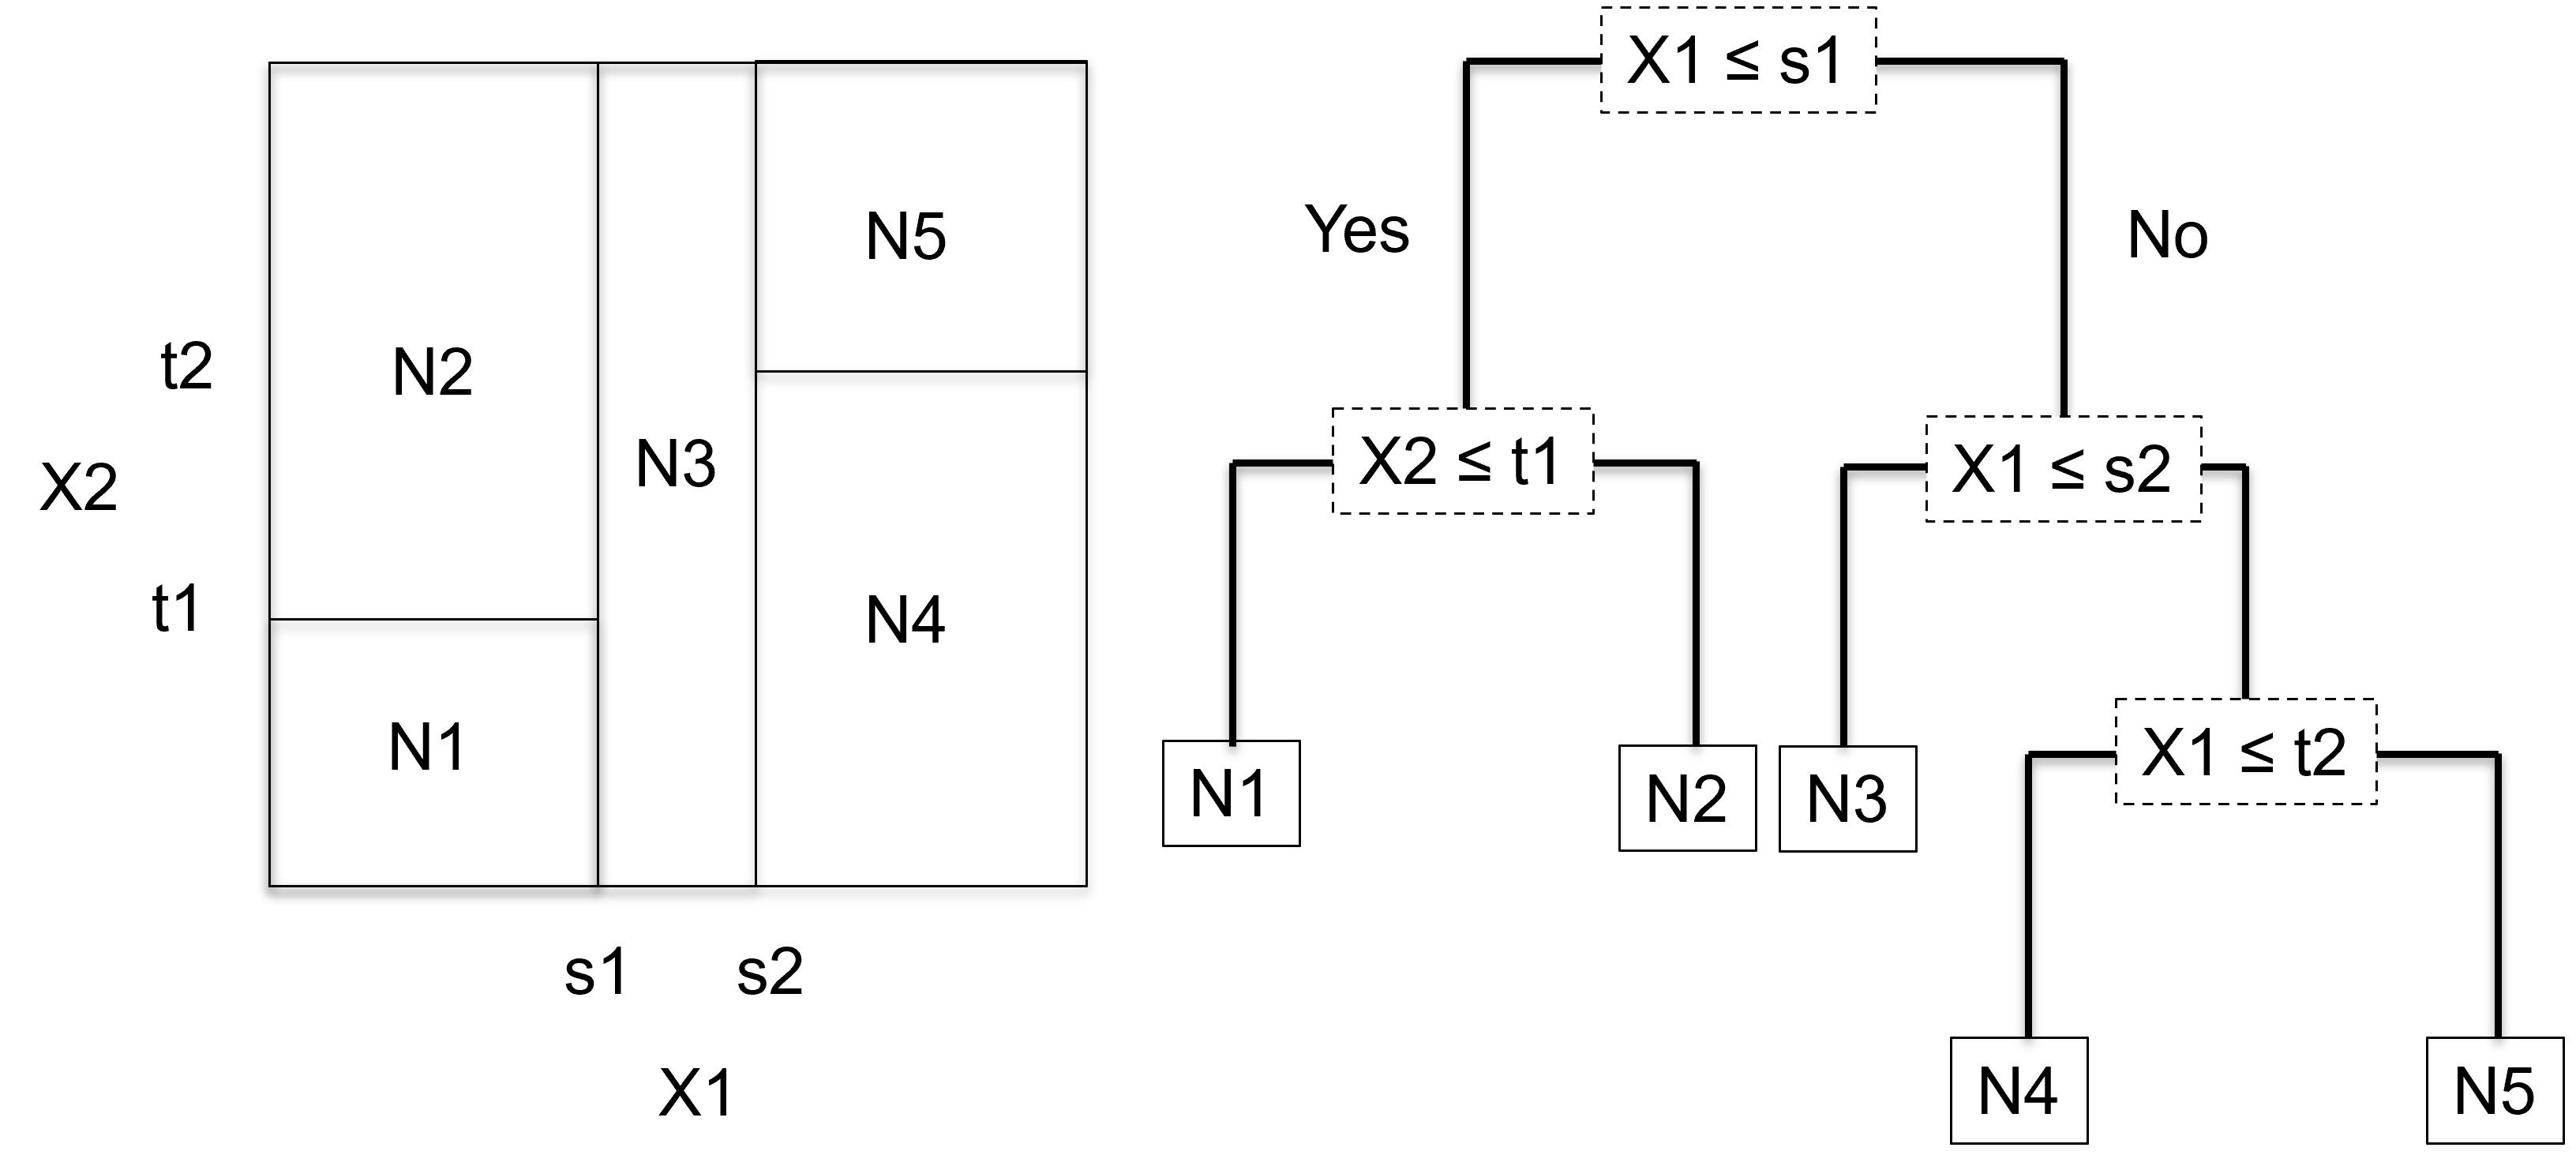
\includegraphics[width=10cm]{../../Graphs/CART_Picture.png}
\end{center}
Each rectangle is associated to one node and one prediction. 
\end{frame}
%%%%%%%%%%%%%%%%%%%%%%%%%%%%%
\begin{frame}
\frametitle{A greedy algorithm}
The greedy algorithm grows the tree step by step as follows:
\begin{itemize}
\item Start with no partition, 
\item Along each feature $x_j$, find the best split of the training set by this feature. This gives $p$ splits (one for each feature).
\item Compare the $p$ splits and select the best one: the one diminishing the loss the most. 
\end{itemize}
You obtain two nodes, $N_1$ and $N_2$, say. Repeat the above rule on each node until a stopping rule is reached (see later).
\end{frame}
%%%%%%%%%%%%%%%%%%%%%%%%%%%%%
\begin{frame}
\frametitle{A greedy algorithm}
Example of classification:
\begin{center}
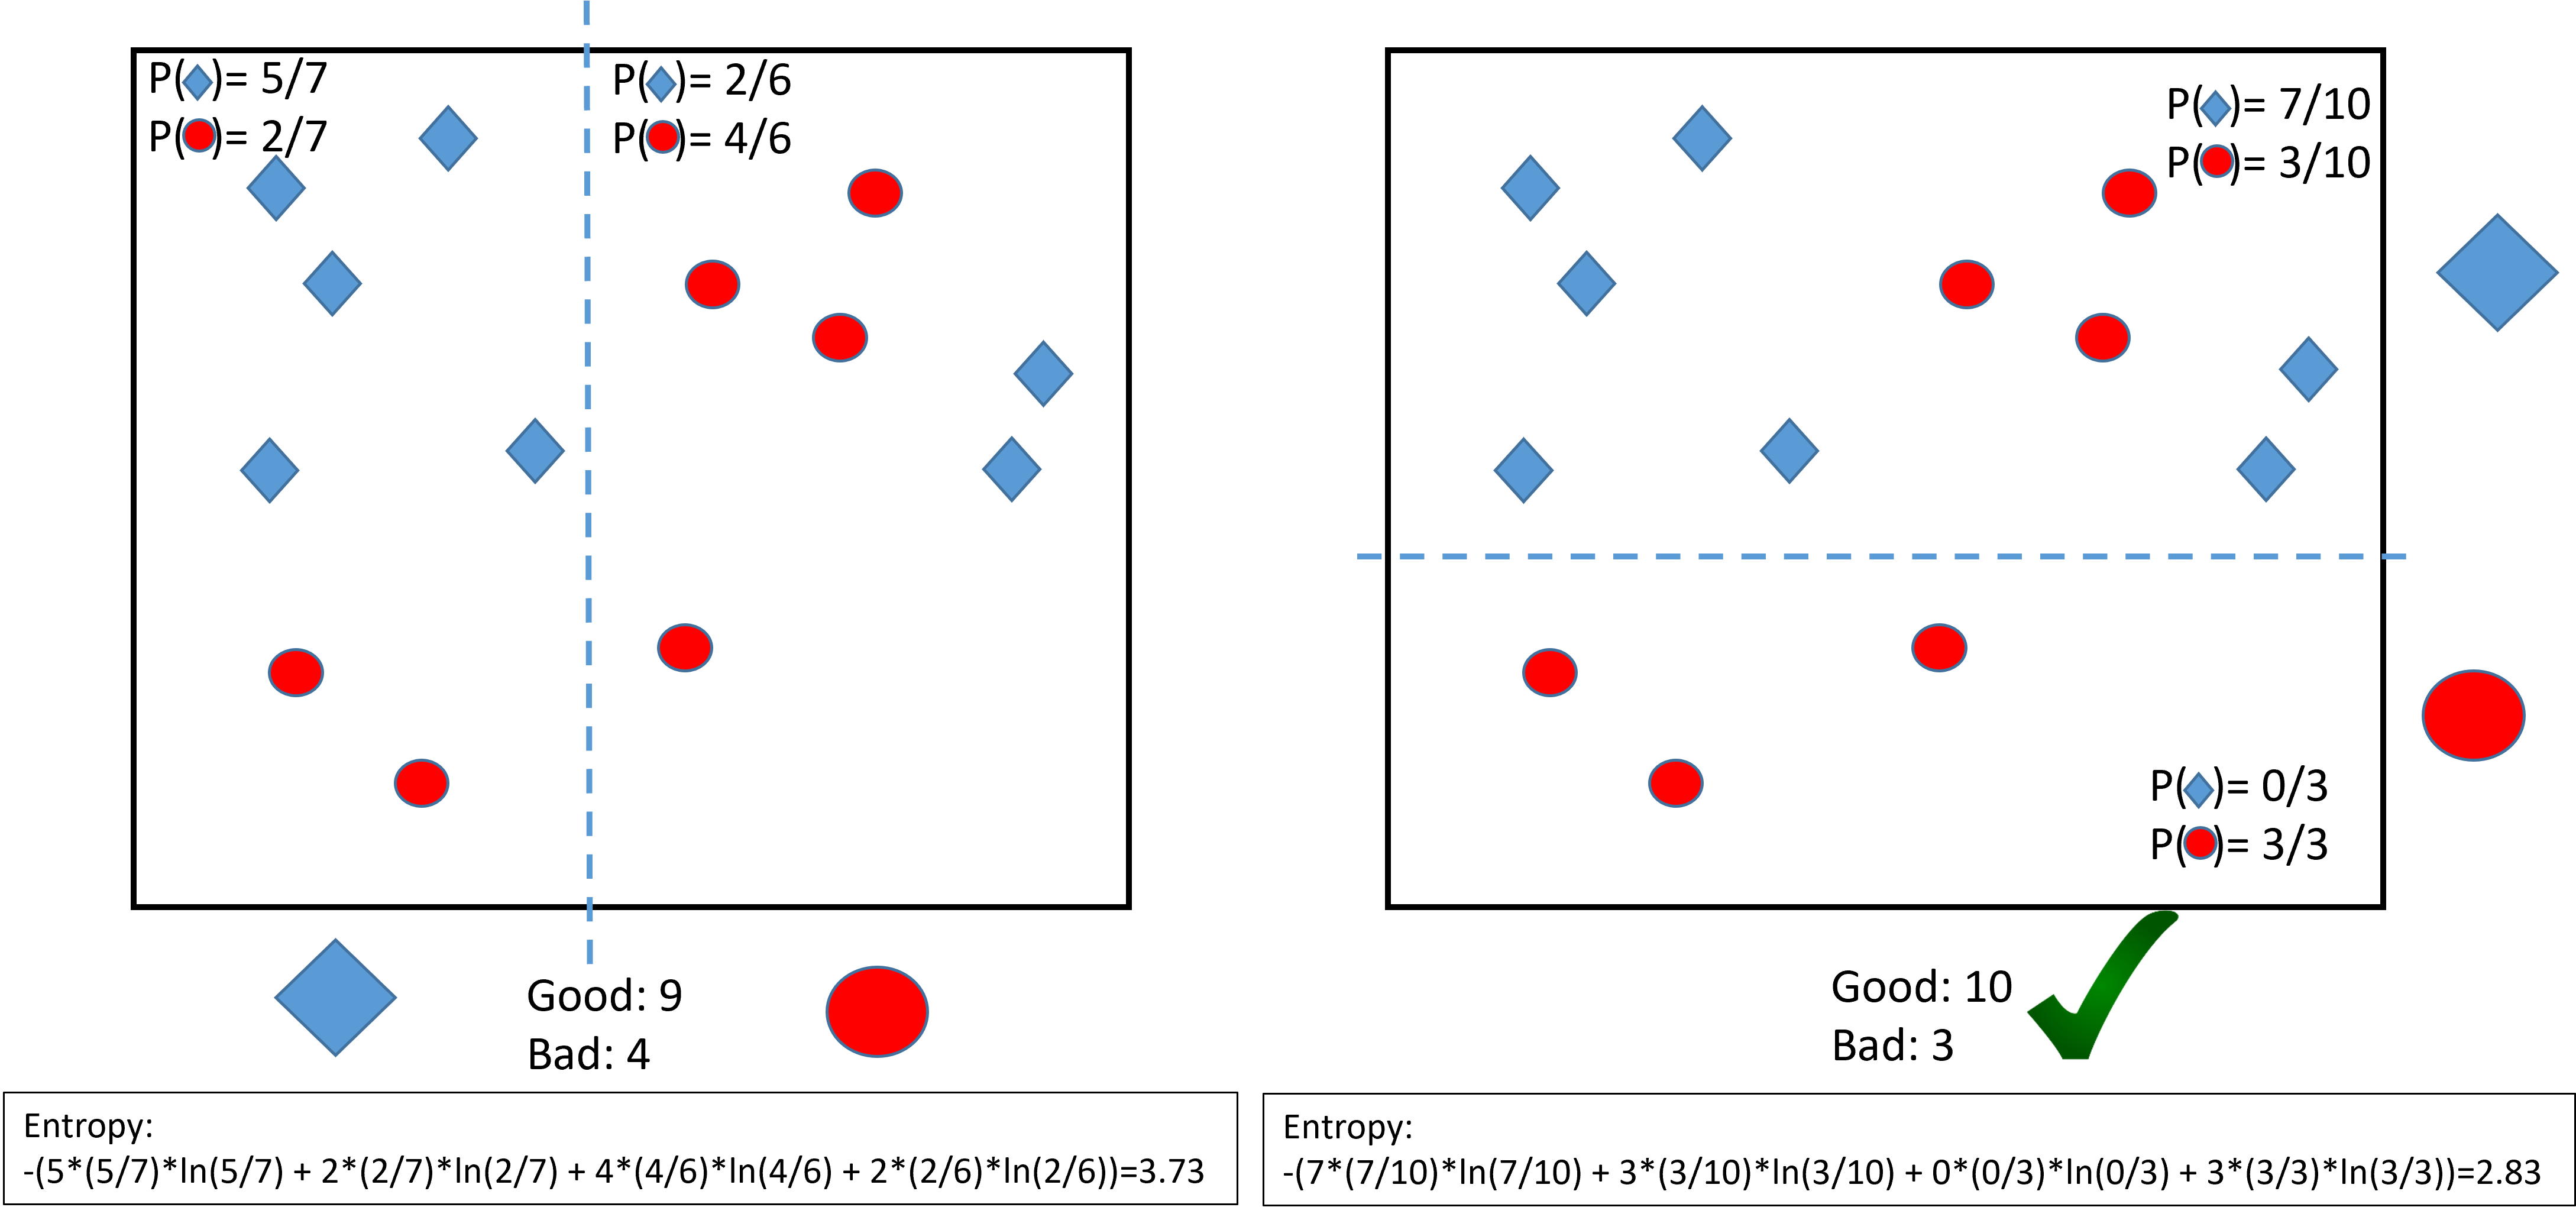
\includegraphics[width=12cm]{../../Graphs/Cart_Build.png}
\end{center}
\scriptsize
Note: by convention $0\times \ln 0 = 0$.
\normalsize
\end{frame}
%%%%%%%%%%%%%%%%%%%%%%%%%%%%%
\begin{frame}
\frametitle{CART: a greedy algorithm}
\begin{center}
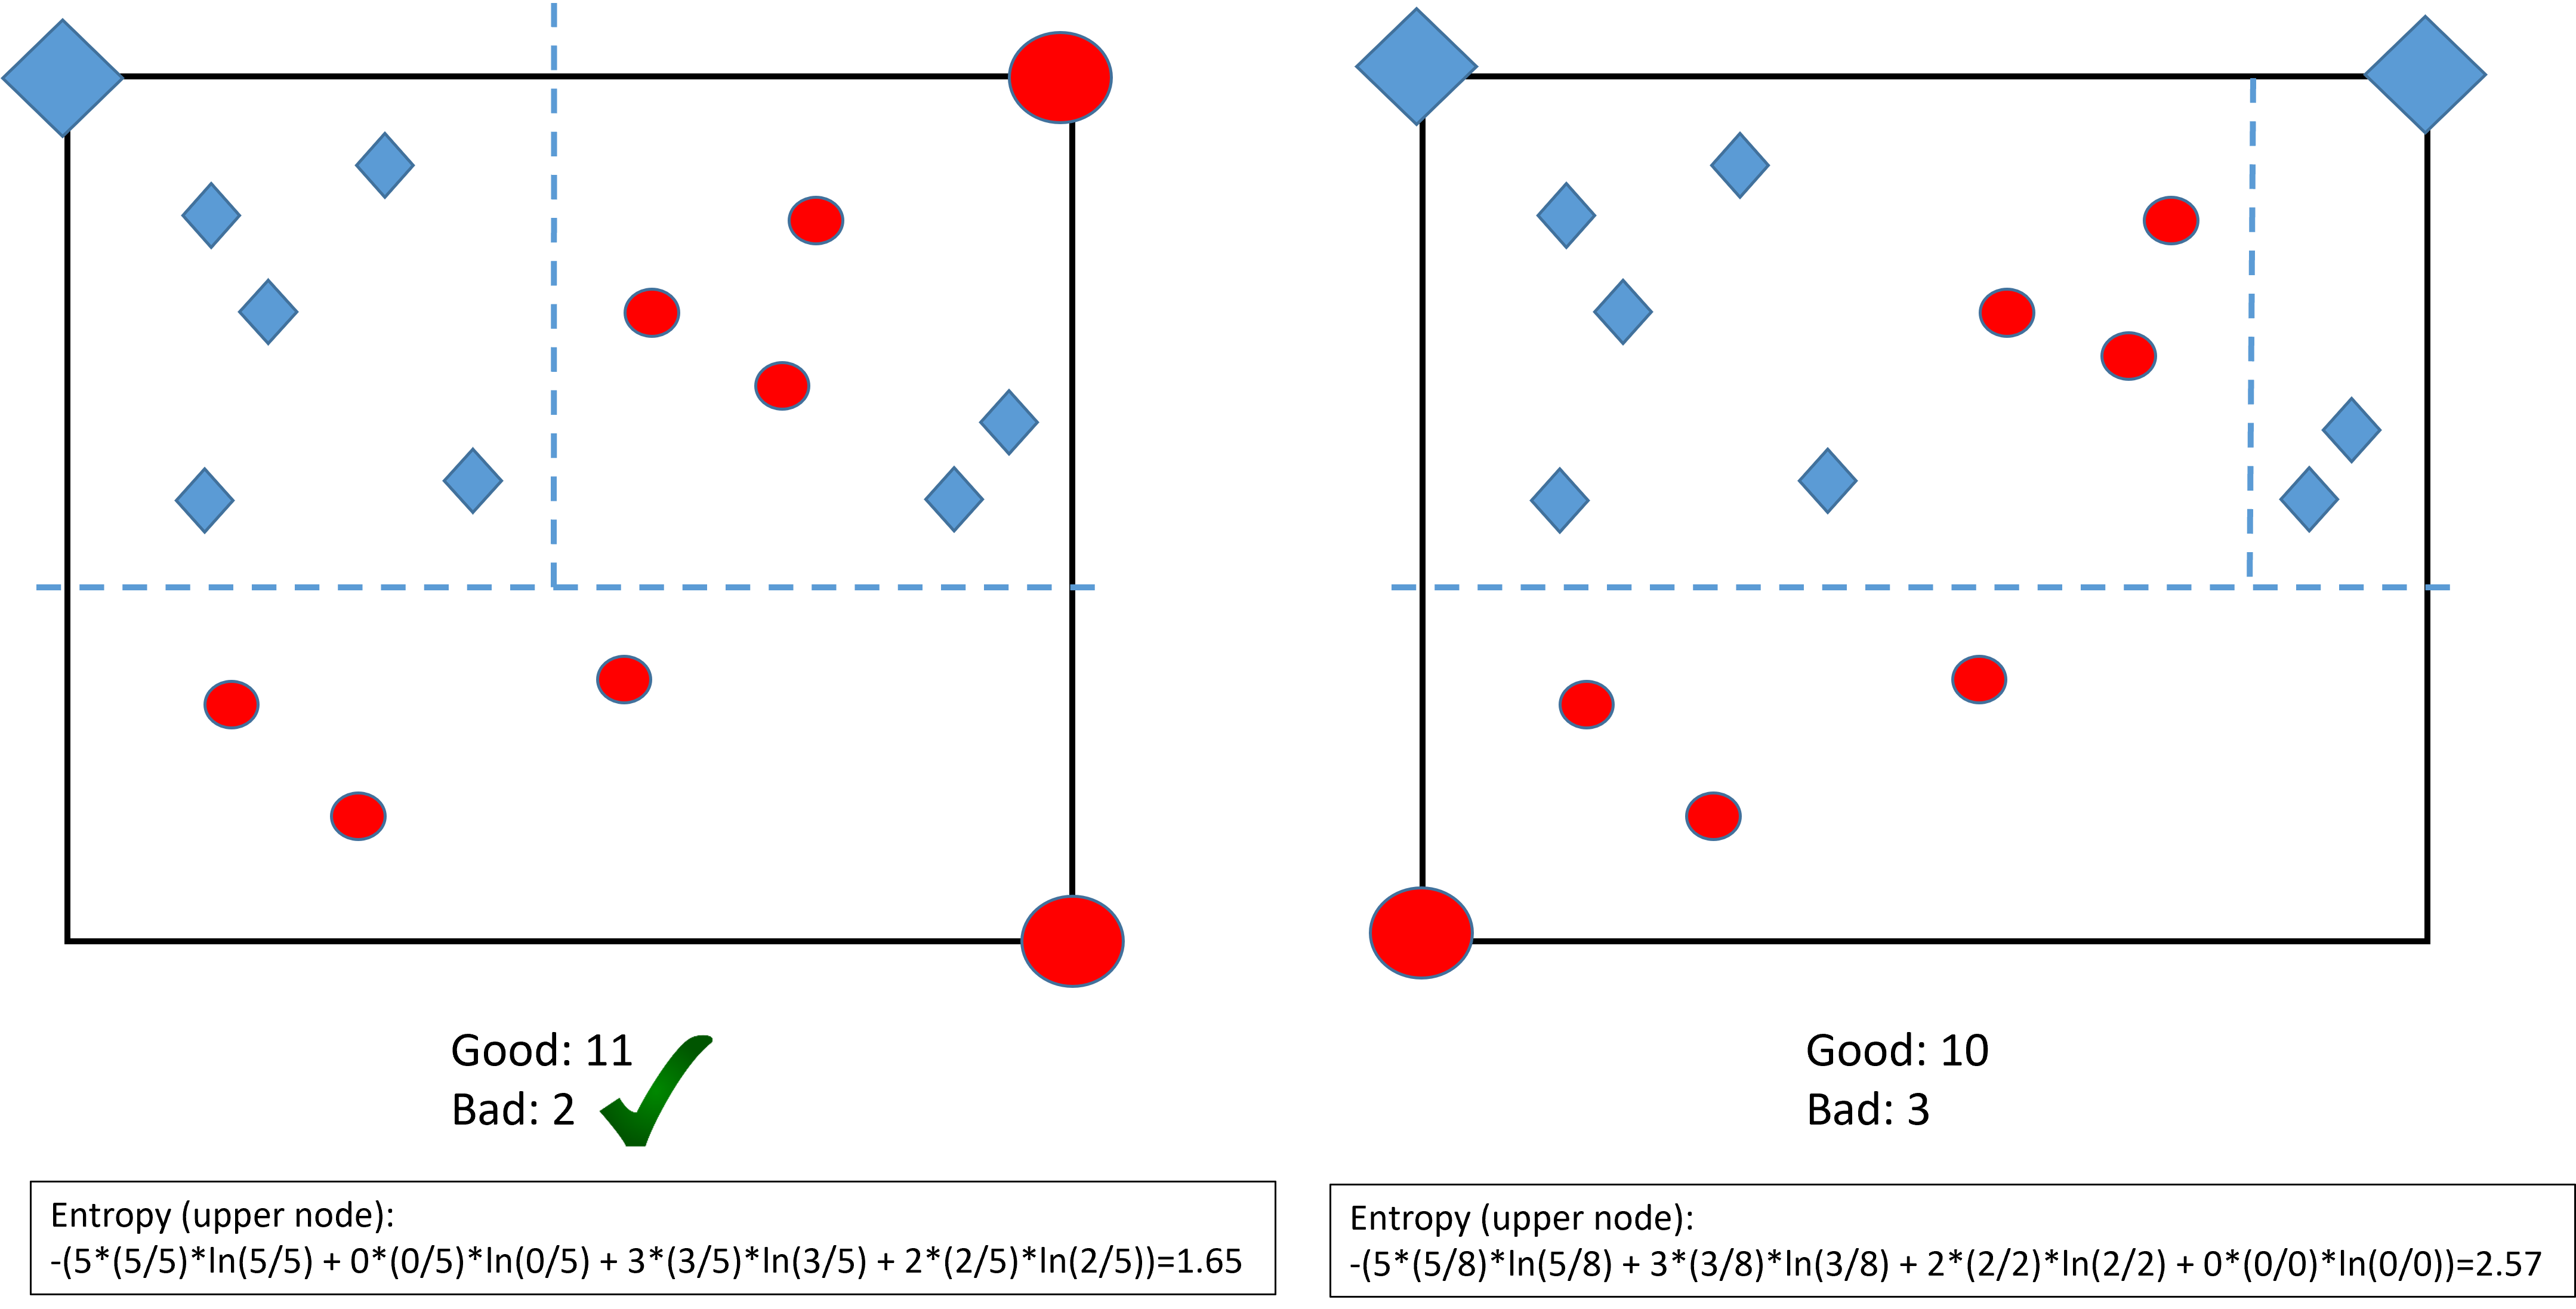
\includegraphics[width=12cm]{../../Graphs/Cart_Build2.png}
\end{center}
etc.
\end{frame}
%%%%%%%%%%%%%%%%%%%%%%%%%%%%%
\begin{frame}
\frametitle{A greedy algorithm}
Example of regression:
\begin{center}
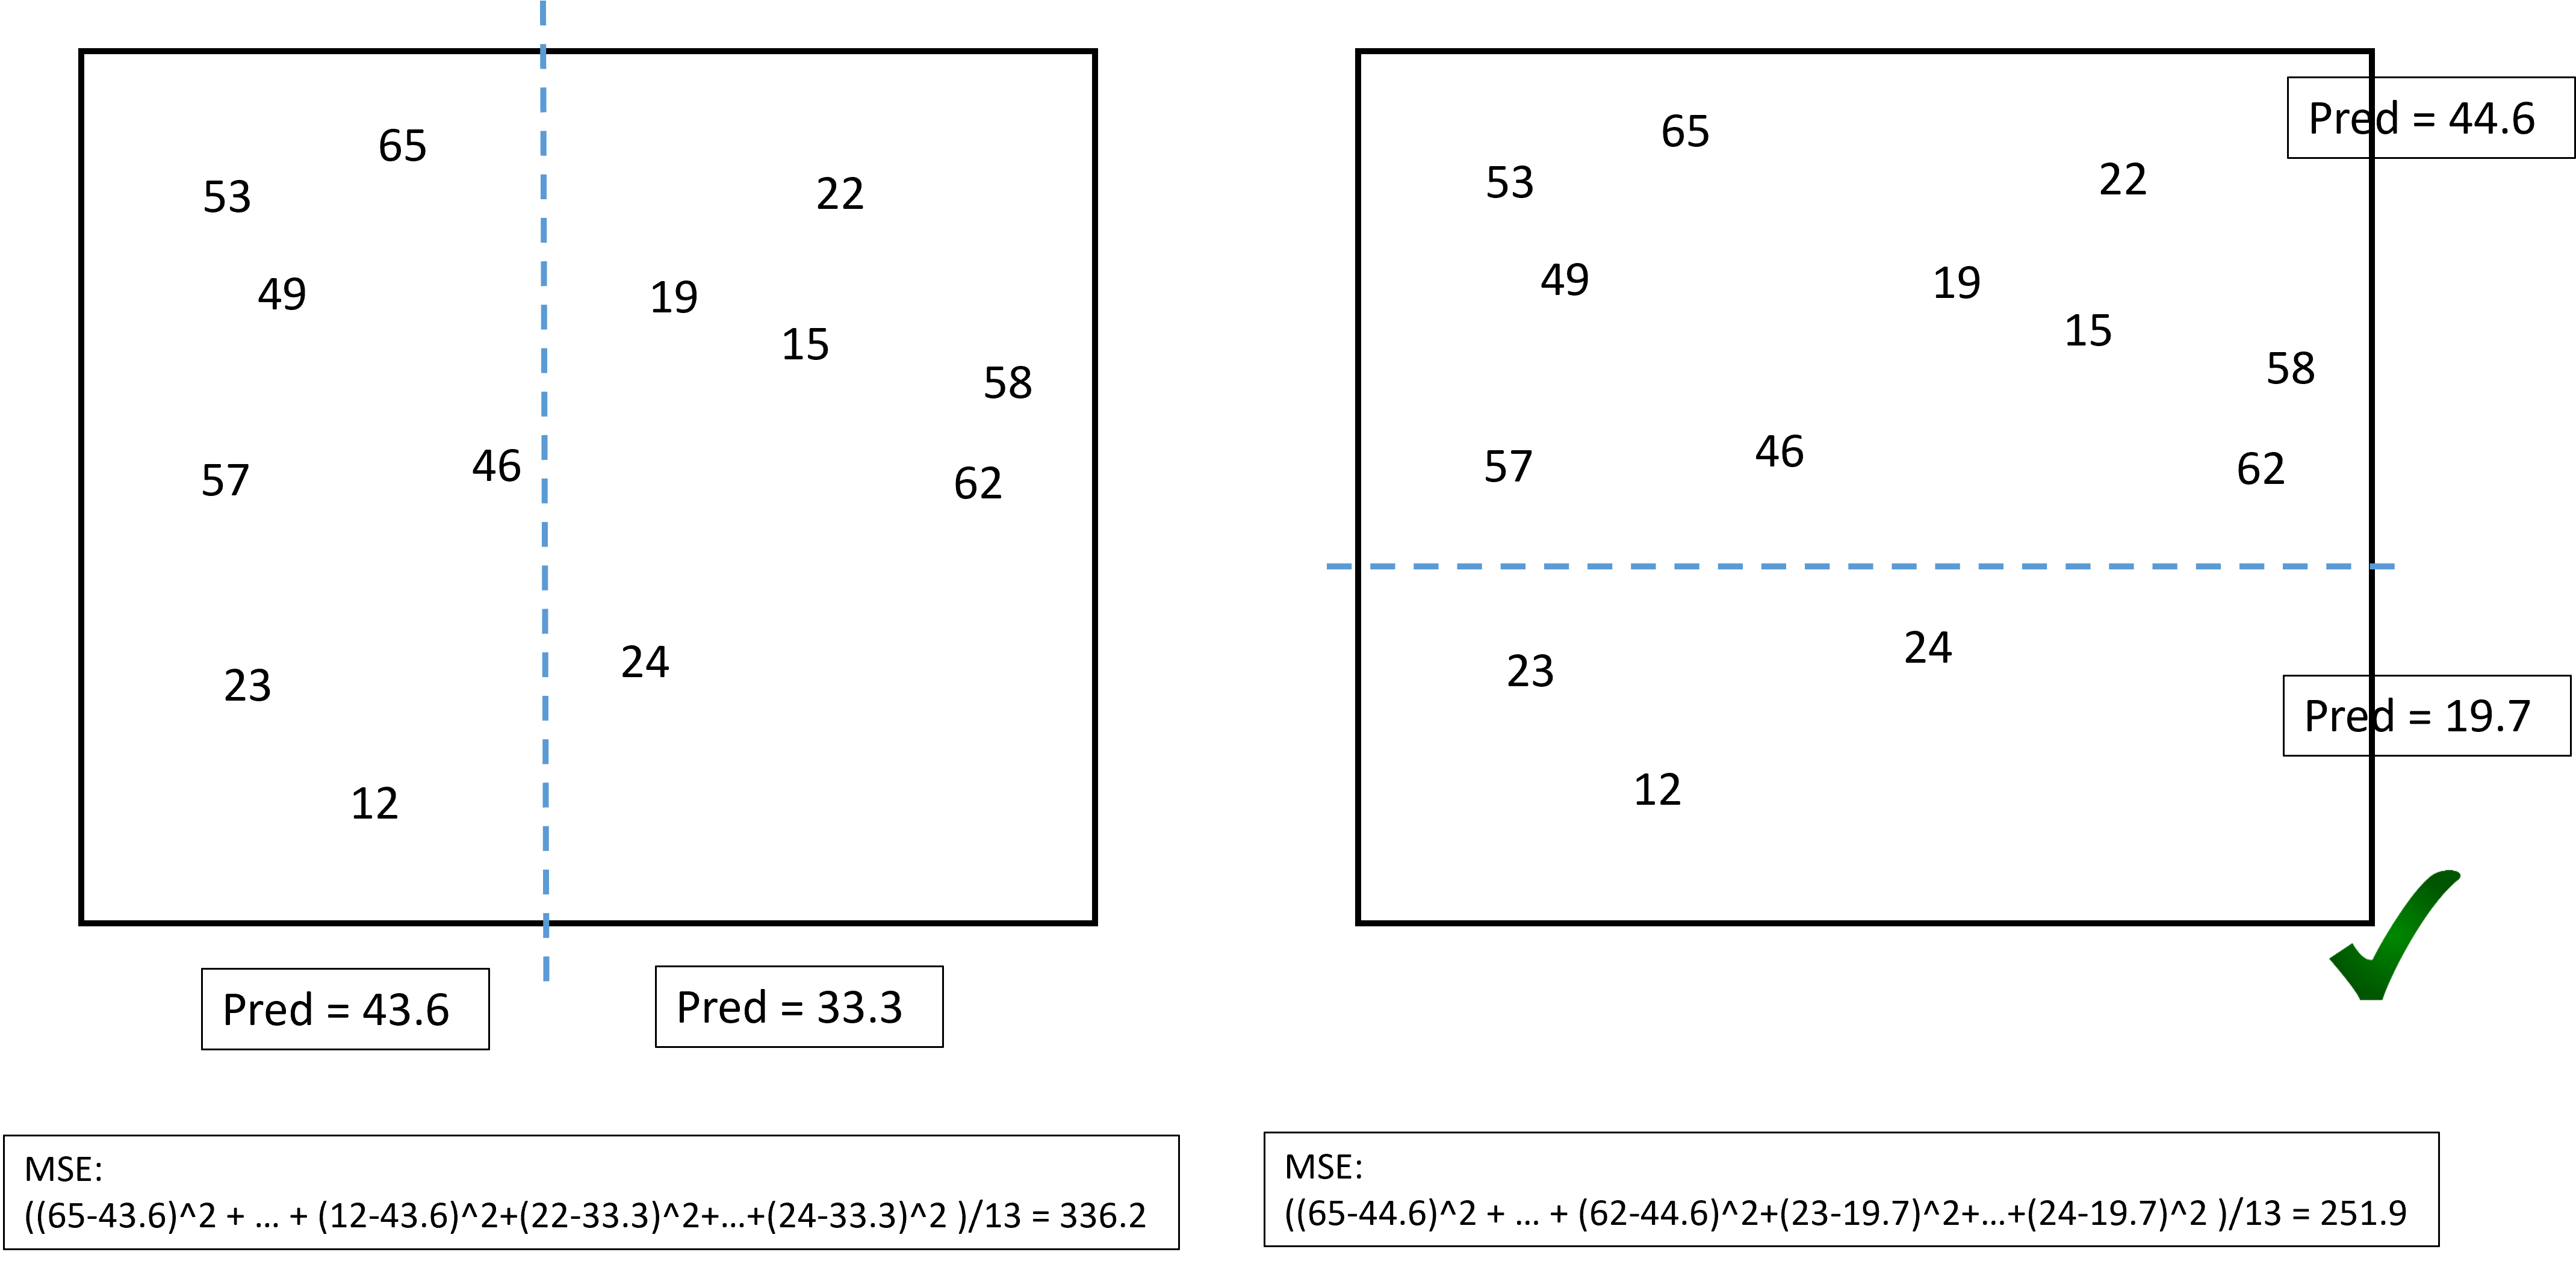
\includegraphics[width=12cm]{../../Graphs/RT_Build.png}
\end{center}
\end{frame}
%%%%%%%%%%%%%%%%%%%%%%%%%%%%%
\begin{frame}
\frametitle{Stopping rule}
The algorithm could go on splitting the feature space forever. Several stopping rules can be used. For example in {\tt R} with {\tt rpart} (see {\tt ?rpart.control}):
\begin{itemize}
\item {\tt minsplit}: the minimum number of observations that must exist in a node in order for a split to be attempted (default is 20).
\item {\tt cp}: Any split that does not decrease the overall lack of fit by a factor of cp is not attempted (default to 0.1).
\item {\tt minbucket}: the minimum number of observations in any terminal node (default to {\tt minsplit/3}).  
\item etc.
\end{itemize}
Even with these rules, once the tree is grown, it might be too large. The procedure of cutting nodes is called {\bf pruning} the tree.  
\end{frame}
%%%%%%%%%%%%%%%%%%%%%%%%%%%%%
\section{Interpretation}
%%%%%%%%%%%%%%%%%%%%%%%%%%%%%
\begin{frame}
\frametitle{Interpretation}
Trees can be interpreted by reading directly on the graph the link between the features and the outcome.
\begin{itemize}
\item The most important feature is at the top of the graph. The first split influence the other ones.
\item The final nodes should be organized in a logical way to ease the reading. E.g., 
\begin{itemize}
\item (regression) Low predictions to the left, high predictions to the right.
\item (binary) predictions "0" to the left, and "1" to the right.
\end{itemize}
\end{itemize}
Interpretation must be done with cautious. \\
\vspace{0.2cm}
The tree structure is unstable: several trees can produce similar predictions. The greedy algorithm may just pick one at random. Repeating the training may lead to a complete different tree.
\end{frame}
%%%%%%%%%%%%%%%%%%%%%%%%%%%%%
\section{Pruning}
%%%%%%%%%%%%%%%%%%%%%%%%%%%%%%%%%%%%%%%%%%%%%
\begin{frame}
\frametitle{Occam's razor}
For linear and logistic regressions, the more variables are in the model, the more complex that model is.\\
\vspace{0.3cm}
For trees, complexity is measured by the length of the tree: a shorter tree is more simple than a longer one.\\
\vspace{0.3cm}
To apply Occan's razor, one needs to shorten the tree without impeding too much its prediction quality.\\
\vspace{0.3cm}
To {\bf prune} the tree consists of cutting branches (i.e., a posteriori) while maintaining enough prediction quality. 
\end{frame}
%%%%%%%%%%%%%%%%%%%%%%%%%%%%%
\begin{frame}
\frametitle{1-SE rule}
There exist several ways to prune the tree. One of the most used is the {\bf 1-SE rule}. 
\begin{itemize}
\item Start with a long tree (using the default stopping rules)
\item For all the sub-trees compute the error of the tree 
\item For the best tree (i.e., with the lowest error), compute the uncertainty on that error measure: the {\bf standard error} SE.
\item Any tree whose error is below the lowest error plus one SE is considered equivalent to the best tree.
\item Select the shortest tree among those that are equivalent to the best one.
\end{itemize}
\end{frame}
%%%%%%%%%%%%%%%%%%%%%%%%%%%%%
\begin{frame}
\frametitle{Technical details}
\begin{itemize}
\item The SE is computed using cross-validation (see later).
\item The 1-SE rule can be replaced by other rules (like cutting at a given CP, etc.). 
\end{itemize}
In practice, 
\begin{itemize}
\item the pruning is not a guarantee to obtain a good model. 
\item It should be used to simplify the model and avoid overfitting.
\item (empirical) it works well to build a very large tree then to prune it.
\end{itemize}
\end{frame}
%%%%%%%%%%%%%%%%%%%%%%%%%%%%%
\end{document}

\begin{frame}
\frametitle{Pruning}
Example {\tt BreastCancer} data set (in {\tt mlbench}).\\
\scriptsize
The objective is to identify each of a number of benign or malignant classes. [...] Each variable except for the first was converted into 11 primitive numerical attributes with values ranging from 0 through 10. 
\normalsize
\begin{center}
\includegraphics[width=6cm]{../../Graphs/BreastCancerLongTree.pdf}
\end{center}
\end{frame}
%%%%%%%%%%%%%%%%%%%%%%%%%%%%%
\begin{frame}
\frametitle{Pruning}
Below, a measure of errors of all the sub-trees and the 1-SE limit from the best tree (size=4). The simplest equivalent to the best tree is of size 3.
\begin{center}
\includegraphics[width=7cm]{../../Graphs/BreastCancer_CPs.pdf}
\end{center}
\end{frame}
%%%%%%%%%%%%%%%%%%%%%%%%%%%%%
\begin{frame}
\frametitle{Pruning}
After the pruning, we will use the tree of size 3.
\begin{center}
\includegraphics[width=7cm]{../../Graphs/BreastCancerShortTree.pdf}
\end{center}
\end{frame}
%%%%%%%%%%%%%%%%%%%%%%%%%%%%%

\begin{frame}
\frametitle{A greedy algorithm}
On the following step, the two splits are built from the previous one. The left one is the best. 
\begin{center}
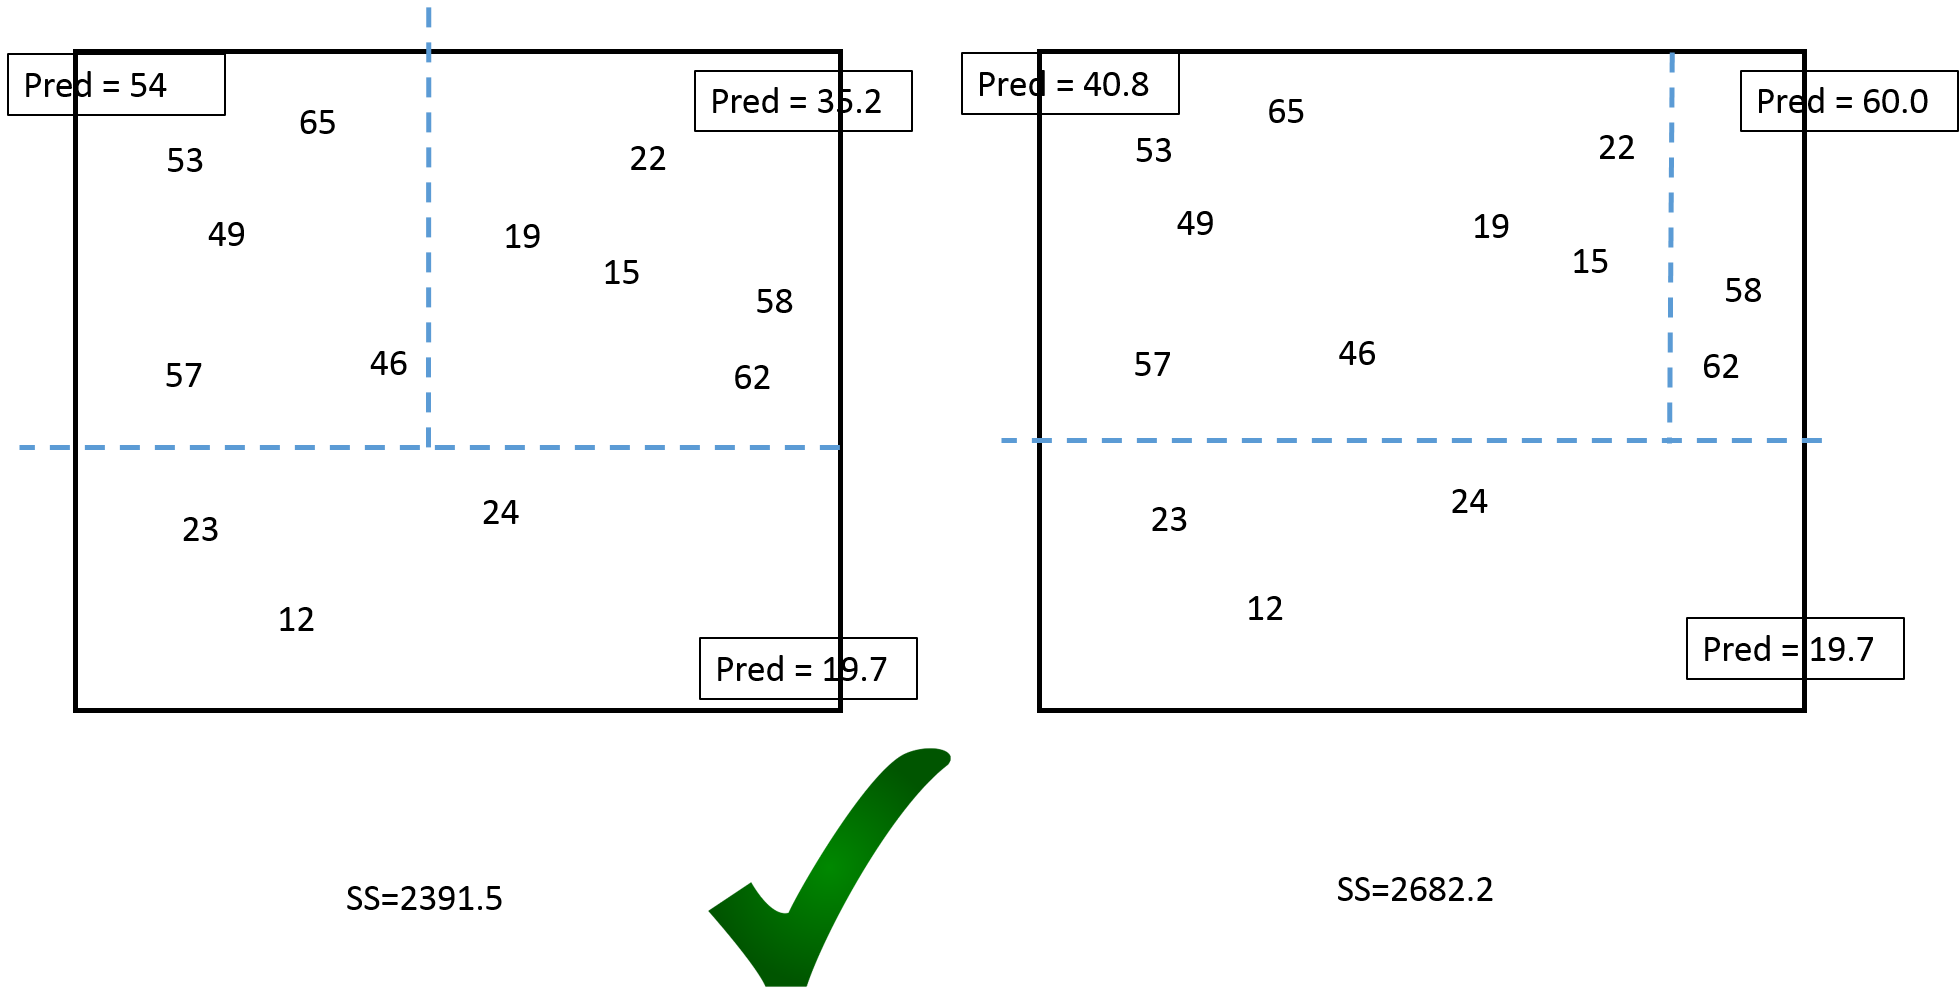
\includegraphics[width=9cm]{../../Graphs/RT_Build2.png}
\end{center}
The construction goes on like for the classification tree.  
\end{frame}
%%%%%%%%%%%%%%%%%%%%%%%%%%%%%
\begin{frame}
\frametitle{Impurity}
\begin{itemize}
\item A {\it good} split is define relative to a criterion of error called {\bf impurity} (measure of bad quality). 
\item A good split minimizes the impurity.
\item The impurity depends on the task: classification or regression.
\end{itemize}
\end{frame}
%%%%%%%%%%%%%%%%%%%%%%%%%%%%%
\begin{frame}
\frametitle{Impurity for classification}
Impurity $Q(D)$, for node $D$, with class prediction $c_D$. Common choices are
\begin{itemize}
\item {\bf Classification error}: 
$$
Q(D)=1-p_{c_D}(D).
$$
\item {\bf Gini index}:
$$
Q(D) = \sum_{c=1}^C p_c(D)\{1-p_c(D)\}.
$$
\item {\bf Entropy}:
$$
Q(D) = -\sum_{c=1}^C p_c(D)\log_2 p_c(D).
$$
\end{itemize}
\vspace{0.2cm} 
where, $p_c(D)$ is the proportion of instances with class $c$ in node a $D$
$$
p_c(D) = \frac{1}{|D|}\sum_{i\in D} 1_{\{y_i = c\}}.
$$
\end{frame}
%%%%%%%%%%%%%%%%%%%%%%%%%%%%%
\begin{frame}
\frametitle{Impurity: example}
Iris example: consider the final nodes from the left ($D_1$) to the right ($D_3$). Then
\begin{columns}
\begin{column}{0.5\textwidth}
\scriptsize
\begin{tabular}{|l|r|r|r|}
\hline
& $p_{\mbox{Set}}(D)$ & $p_{\mbox{Ver}}(D)$ & $p_{\mbox{Vir}}(D)$ \\
\hline
$D_1$ (Set) & $35/35$ & $0/35$ & $0/35$\\
\hline
$D_2$ (Ver) & $0/34$ & $33/34$ & $1/34$\\
\hline
$D_3$ (Vir) & $0/36$ & $2/36$ & $34/36$\\
\hline
\end{tabular}
\normalsize
\end{column}
\begin{column}{0.5\textwidth}
\begin{center}
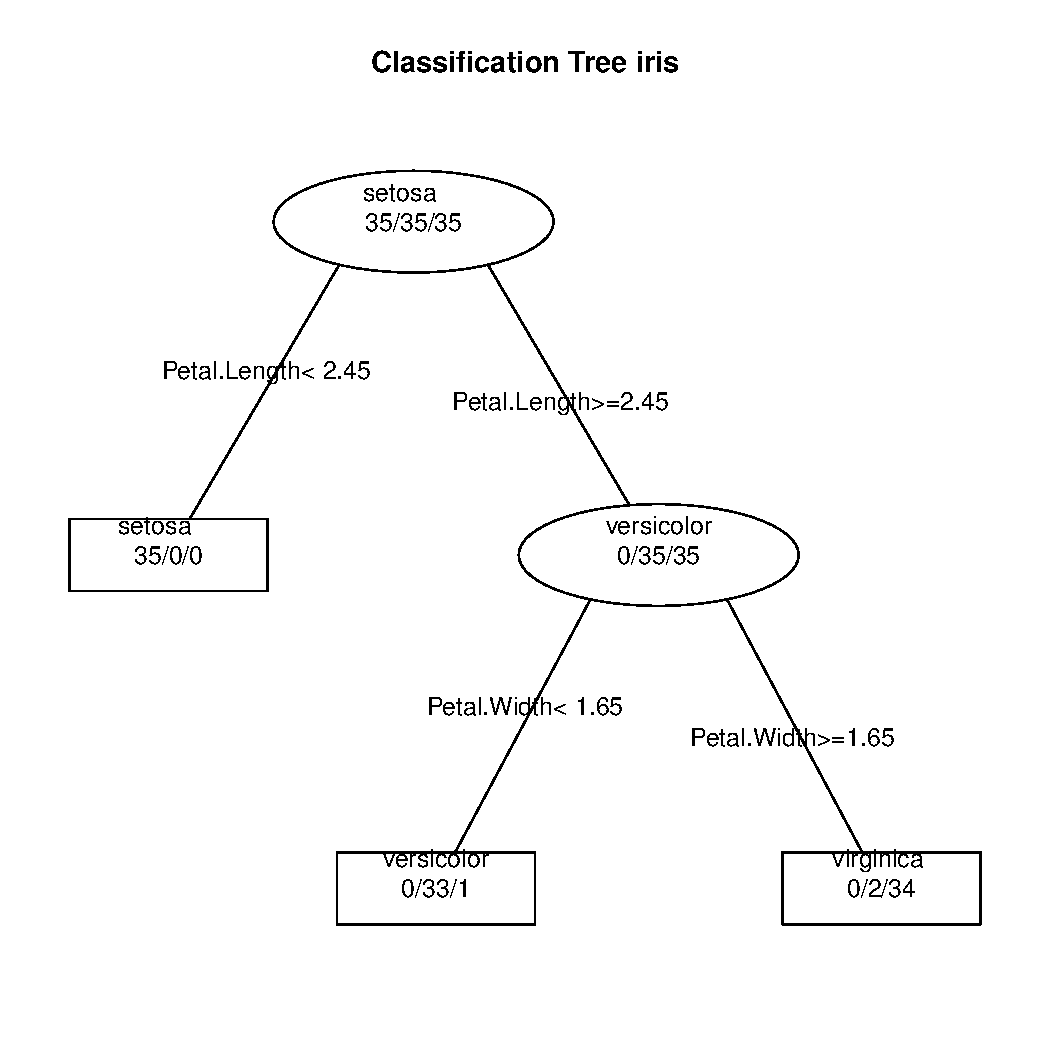
\includegraphics[width=5cm]{../../Graphs/IRIS_CART.pdf}
\end{center}
\end{column}
\end{columns}
\end{frame}
%%%%%%%%%%%%%%%%%%%%%%%%%%%%%
\begin{frame}
\frametitle{Impurity: example}
\begin{itemize}
\item Classification error for $D_3$:  
\begin{eqnarray*}
c(D_3)= \mbox{Vir}, \quad Q(D_3)= 1 - 34/36 = 1/18.\\
\end{eqnarray*}
\item Gini index for $D_3$:
\begin{eqnarray*}
Q(D_3)&=& \frac{0}{36}\times\left(1-\frac{36}{36}\right) + \frac{2}{36}\times\left(1-\frac{34}{36}\right) + \frac{34}{36}\times \left(1-\frac{2}{36}\right)\\
&=& \frac{0}{36}\times\frac{36}{36} + \frac{2}{36}\times\frac{34}{36} + \frac{34}{36}\times\frac{2}{36}\\
&=& 0.105\\
\end{eqnarray*}
\end{itemize}
\end{frame}
%%%%%%%%%%%%%%%%%%%%%%%%%%%%%
\begin{frame}
\frametitle{Impurity: example}
\begin{itemize}
\item Entropy for $D_3$:
\begin{eqnarray*}
Q(D_3)= -0\log_2(0)-\frac{2}{36}\log_2\frac{2}{36} - \frac{34}{36}\log_2\frac{34}{36}=0.31\\
\end{eqnarray*}
\end{itemize}
A "random" node with $(12/36, 12/36, 12/36)$ would have a Gini index of $0.67$ and an entropy of $1.58$. The lower the Gini index / entropy, the better the node.
\end{frame}
%%%%%%%%%%%%%%%%%%%%%%%%%%%%%
\begin{frame}
\frametitle{Impurity for regression}
In regression, most of the time, the impurity is the {\bf mean squared error} (MSE)
$$
Q(D) = \frac{1}{|D|} \sum_{i\in D}(y_i - c_D)^2.
$$
\end{frame}
%%%%%%%%%%%%%%%%%%%%%%%%%%%%%
\begin{frame}
\frametitle{Impurity}
Finally, for the whole tree ${\T}$ made of all the (final) nodes $D \in \T$, then the impurity of the tree is the total impurity of its nodes, weighted by their size:
$$
C(\T) = \sum_{D \in \T} |D| Q(D).
$$
A split is validated when it decreases the impurity of the tree.\\
\end{frame}
%%%%%%%%%%%%%%%%%%%%%%%%%%%%%
\begin{frame}
\frametitle{Stopping the growth}
The algorithm could go on splitting forever without stopping rules. Several rules can be used. For example in {\tt R} with {\tt rpart} (see {\tt ?rpart.control}):
\begin{itemize}
\item {\tt minsplit}: the minimum number of observations that must exist in a node in order for a split to be attempted (default is 20).
\item {\tt cp}: Any split that does not decrease the overall lack of fit by a factor of cp is not attempted (default to 0.1).
\item {\tt minbucket}: the minimum number of observations in any terminal node (default to {\tt minsplit/3}).  
\item etc.
\end{itemize}
Even with these rules, once the tree is grown, it might be too large. The procedure of cutting nodes is called {\tt pruning} the tree.  
\end{frame}
%%%%%%%%%%%%%%%%%%%%%%%%%%%%%
\begin{frame}
\frametitle{Decision rule: regression}
On the Facebook data taking the log of {\tt Lifetime.Post.Consumers} as the outcome.
\begin{center}
\includegraphics[width=10cm]{../../Graphs/FB_RT.png}
\end{center}
\end{frame}
%%%%%%%%%%%%%%%%%%%%%%%%%%%%%
\begin{frame}
\frametitle{Decision rule: regression}
On the Facebook data taking the log of {\tt Lifetime.Post.Consumers} as the outcome.
\begin{center}
\includegraphics[width=10cm]{../../Graphs/FB_RT.png}
\end{center}
\end{frame}
%%%%%%%%%%%%%%%%%%%%%%%%%%%%%
\section{Greedy algorithm}
%%%%%%%%%%%%%%%%%%%%%%%%%%%%%
\begin{frame}
\frametitle{Splitting the data space}
The tree splits the space in rectangles. Below with two features:
\begin{center}
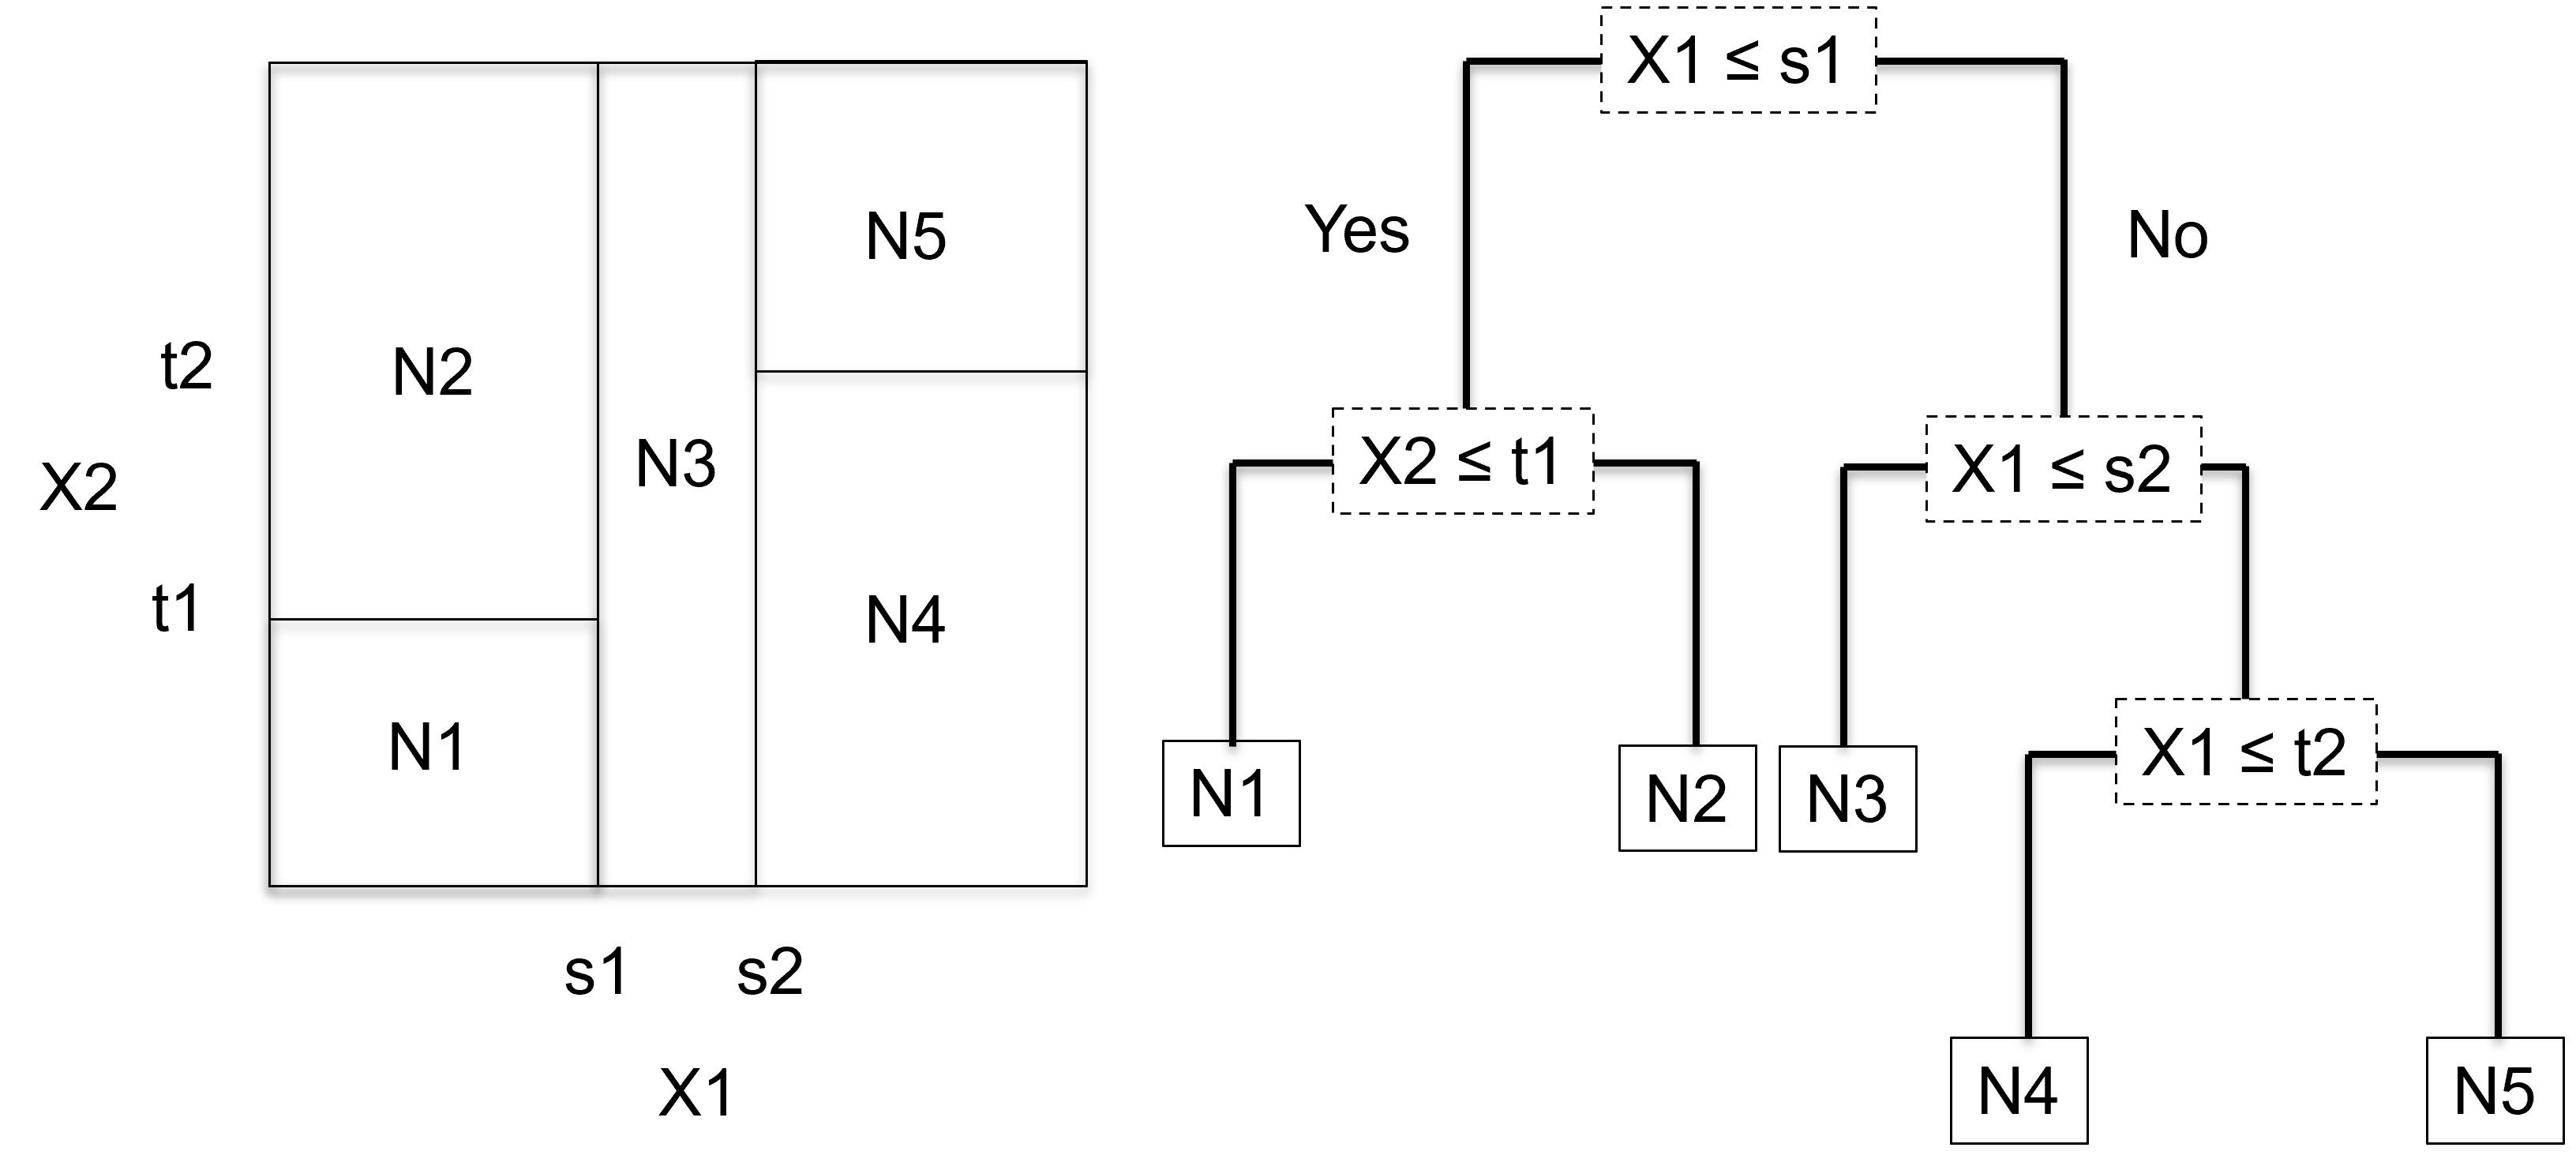
\includegraphics[width=10cm]{../../Graphs/CART_Picture.png}
\end{center}
Each rectangle is associated to one outcome. Several trees may be equivalent.
\end{frame}
%%%%%%%%%%%%%%%%%%%%%%%%%%%%%
\begin{frame}
\frametitle{A greedy algorithm}
To find the optimum partition is computationally infeasible: too many possibilities. One (sub-optimal) solution is to grow the tree step by step: greedy algorithm.
\begin{itemize}
\item Start with no partition, 
\item For each $x_j$, find the best split of the training set by $x_j$.
\item Select the best split over all $x_j$.  
\end{itemize}
You obtain two sets, say $D_1$ and $D_2$, called nodes. Repeat the above rule on each node until a stopping rule is reached.\\
\vspace{0.5cm}
\centerline{What is a "good split"?}
\end{frame}
%%%%%%%%%%%%%%%%%%%%%%%%%%%%%
\begin{frame}
\frametitle{A greedy algorithm}
A split along $x_j$ is a rule of prediction, with two classes $c_1$ and $c_2$ and one threshold $s$:
$$
\hat{y} = \left\{ 
\begin{array}{ll}
c_1, & \mbox{if } x_{j} \leq s,\\
c_2, & \mbox{if } x_{j} > s.
\end{array}\right.
$$
Where $c_1$ and $c_2$ are 
\begin{itemize}
\item (classification) the most frequent class in each side of $s$. 
\item (regression) the average of the outcome in each side of $s$.
\end{itemize}
Ties are often resolved at random.\\
%\vspace{0.2cm}
%{\bf Example}: 
%\begin{itemize}
%\item The first split is along Petal length ($x_3$) with $s=2.45$. $c_1$ is setosa and $c_2$ is versicolor (chosen at random). 
%\item The second split: the node "versicolor" is split along Petal width at $s=1.65$.
%\end{itemize}
\end{frame}
%%%%%%%%%%%%%%%%%%%%%%%%%%%%%
\begin{frame}
\frametitle{A greedy algorithm}
Example of classification:
\begin{center}
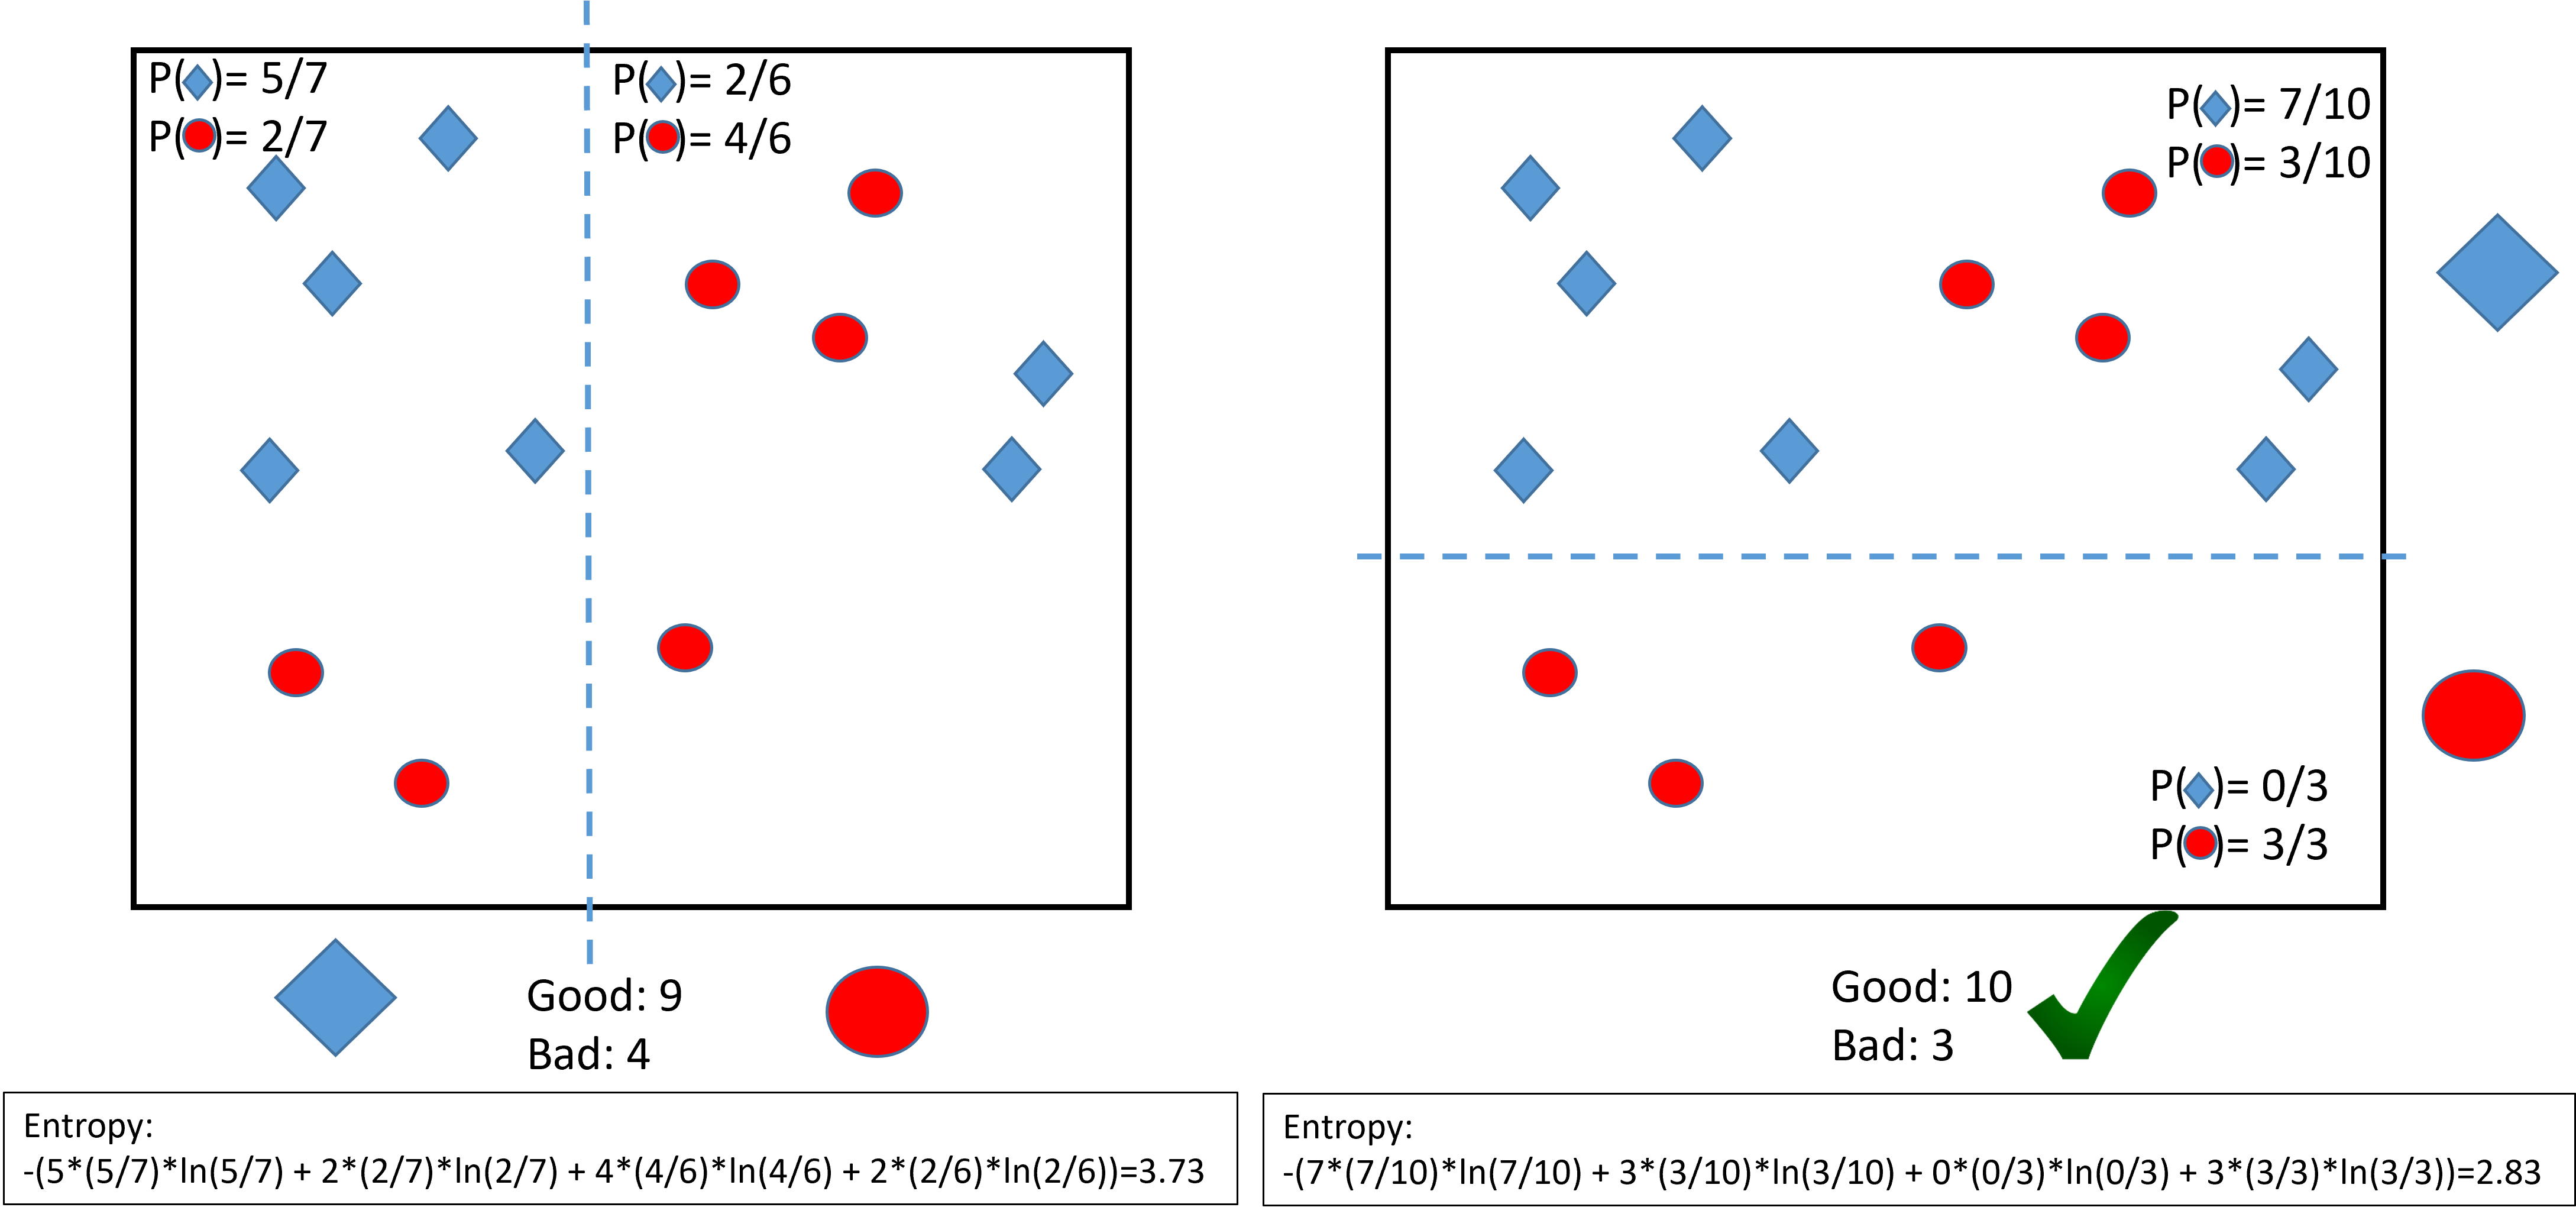
\includegraphics[width=10cm]{../../Graphs/Cart_Build.png}
\end{center}
\end{frame}
%%%%%%%%%%%%%%%%%%%%%%%%%%%%%
\begin{frame}
\frametitle{CART: a greedy algorithm}
\begin{center}
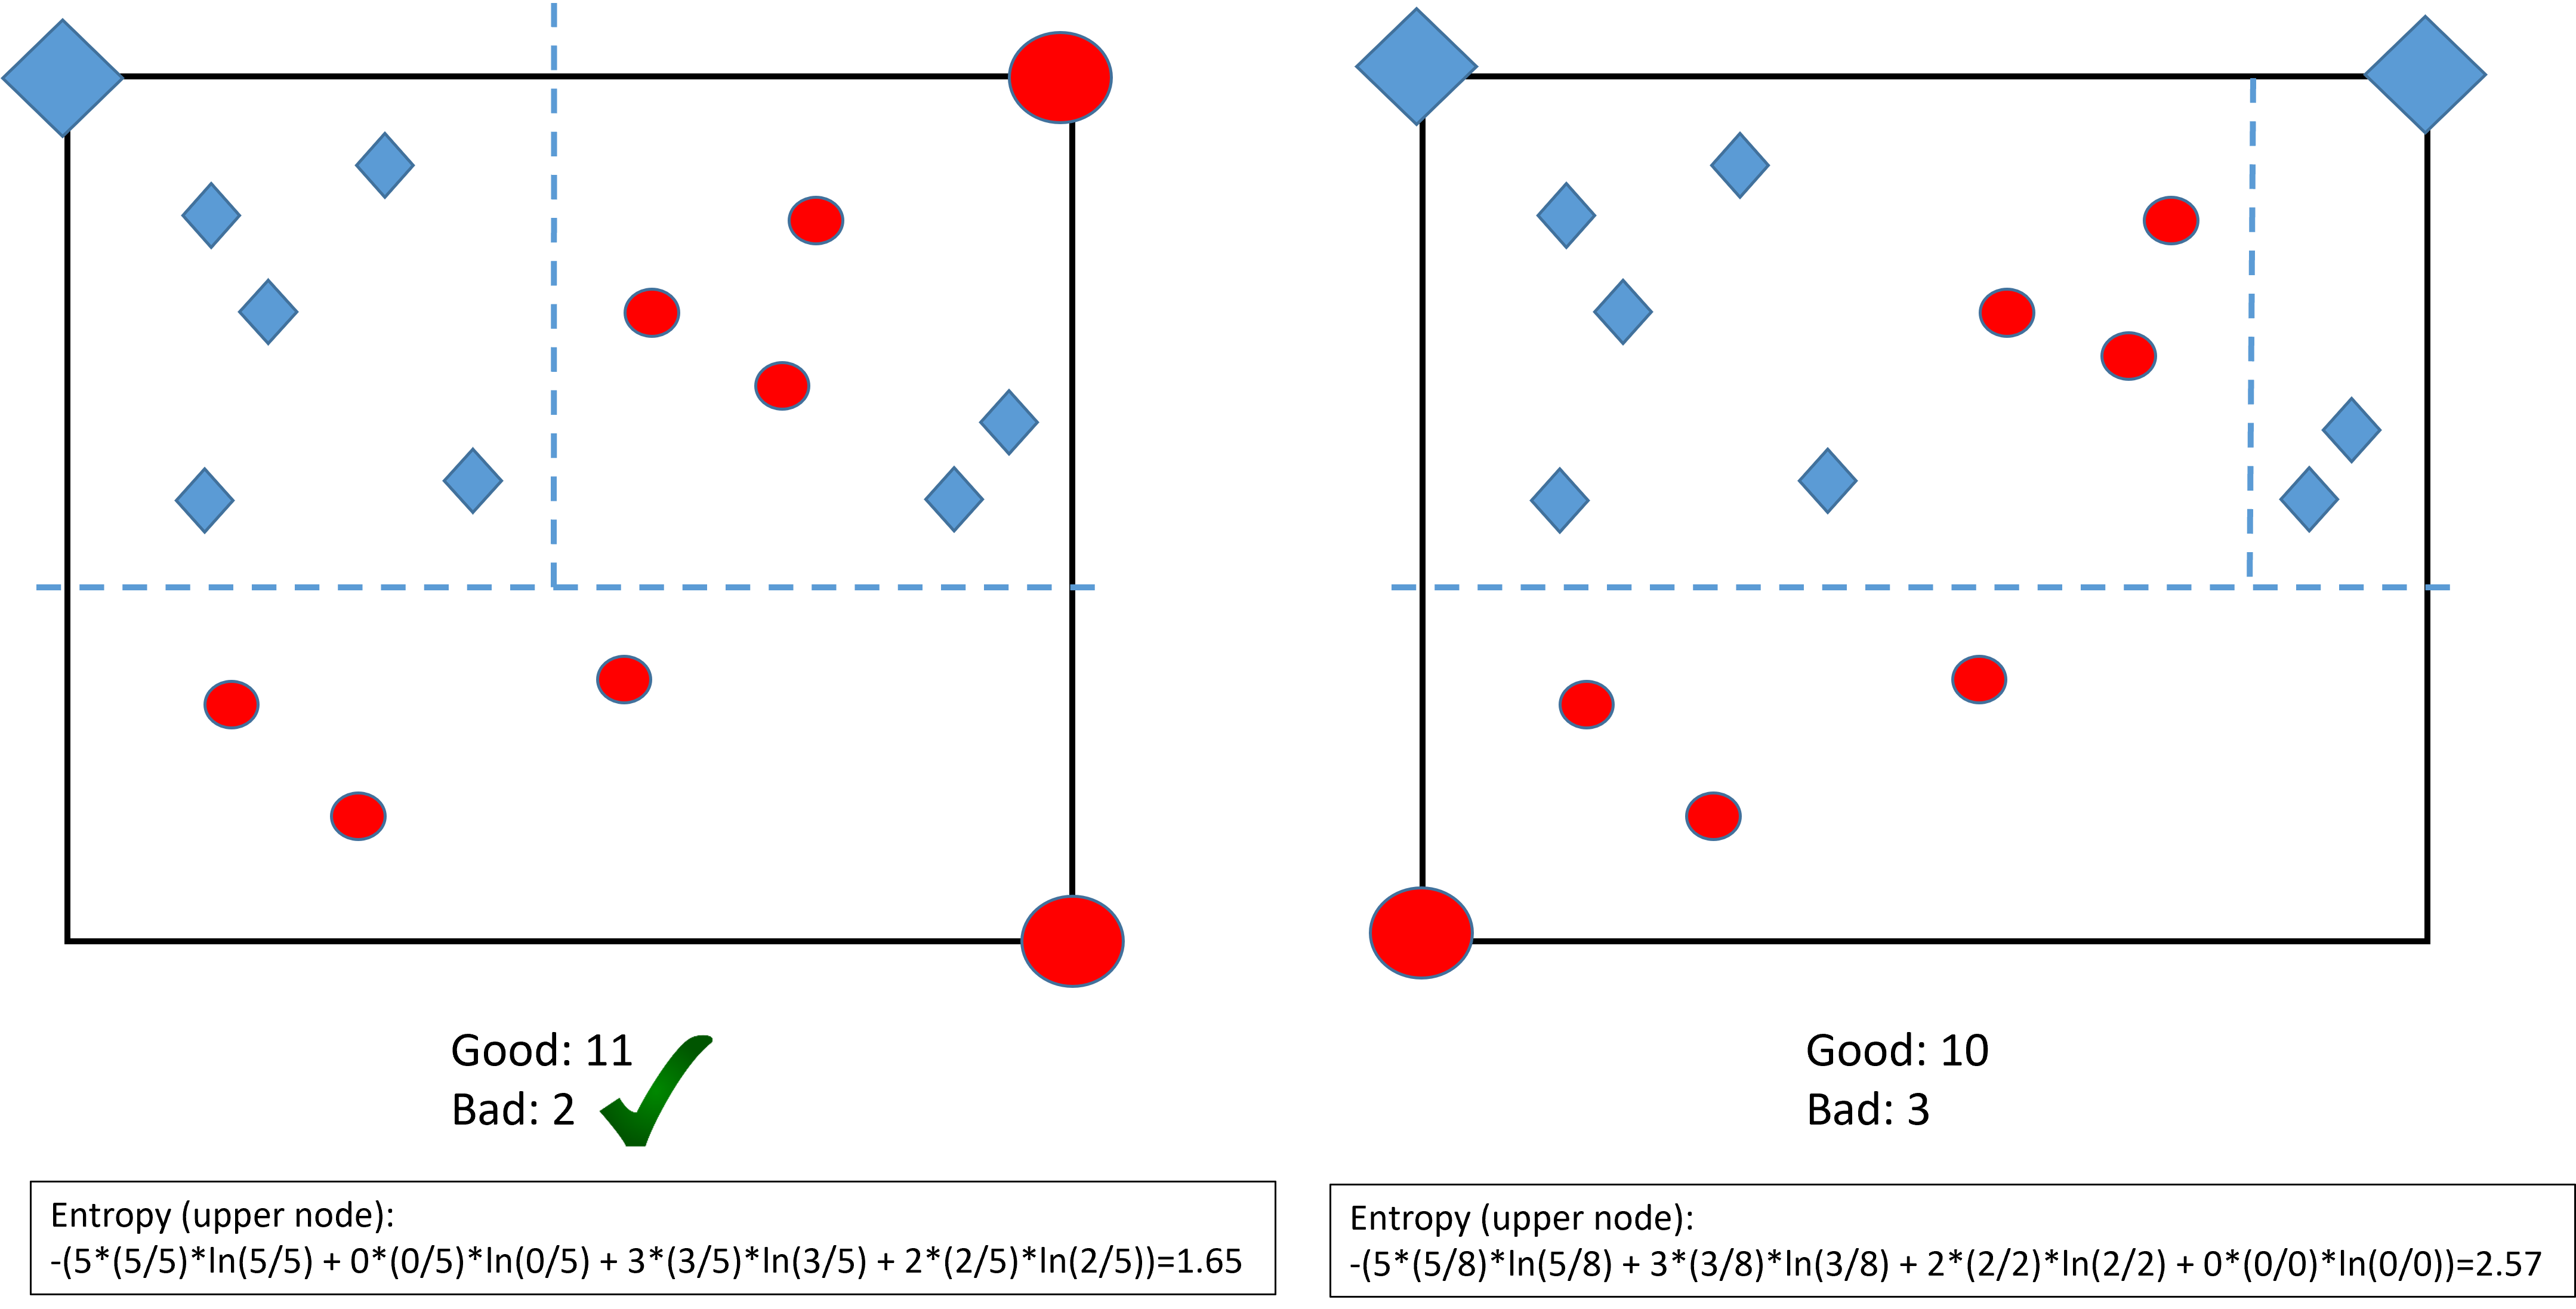
\includegraphics[width=10cm]{../../Graphs/Cart_Build2.png}
\end{center}
etc.
\end{frame}
%%%%%%%%%%%%%%%%%%%%%%%%%%%%%
\begin{frame}
\frametitle{A greedy algorithm}
Example of regression:
\begin{center}
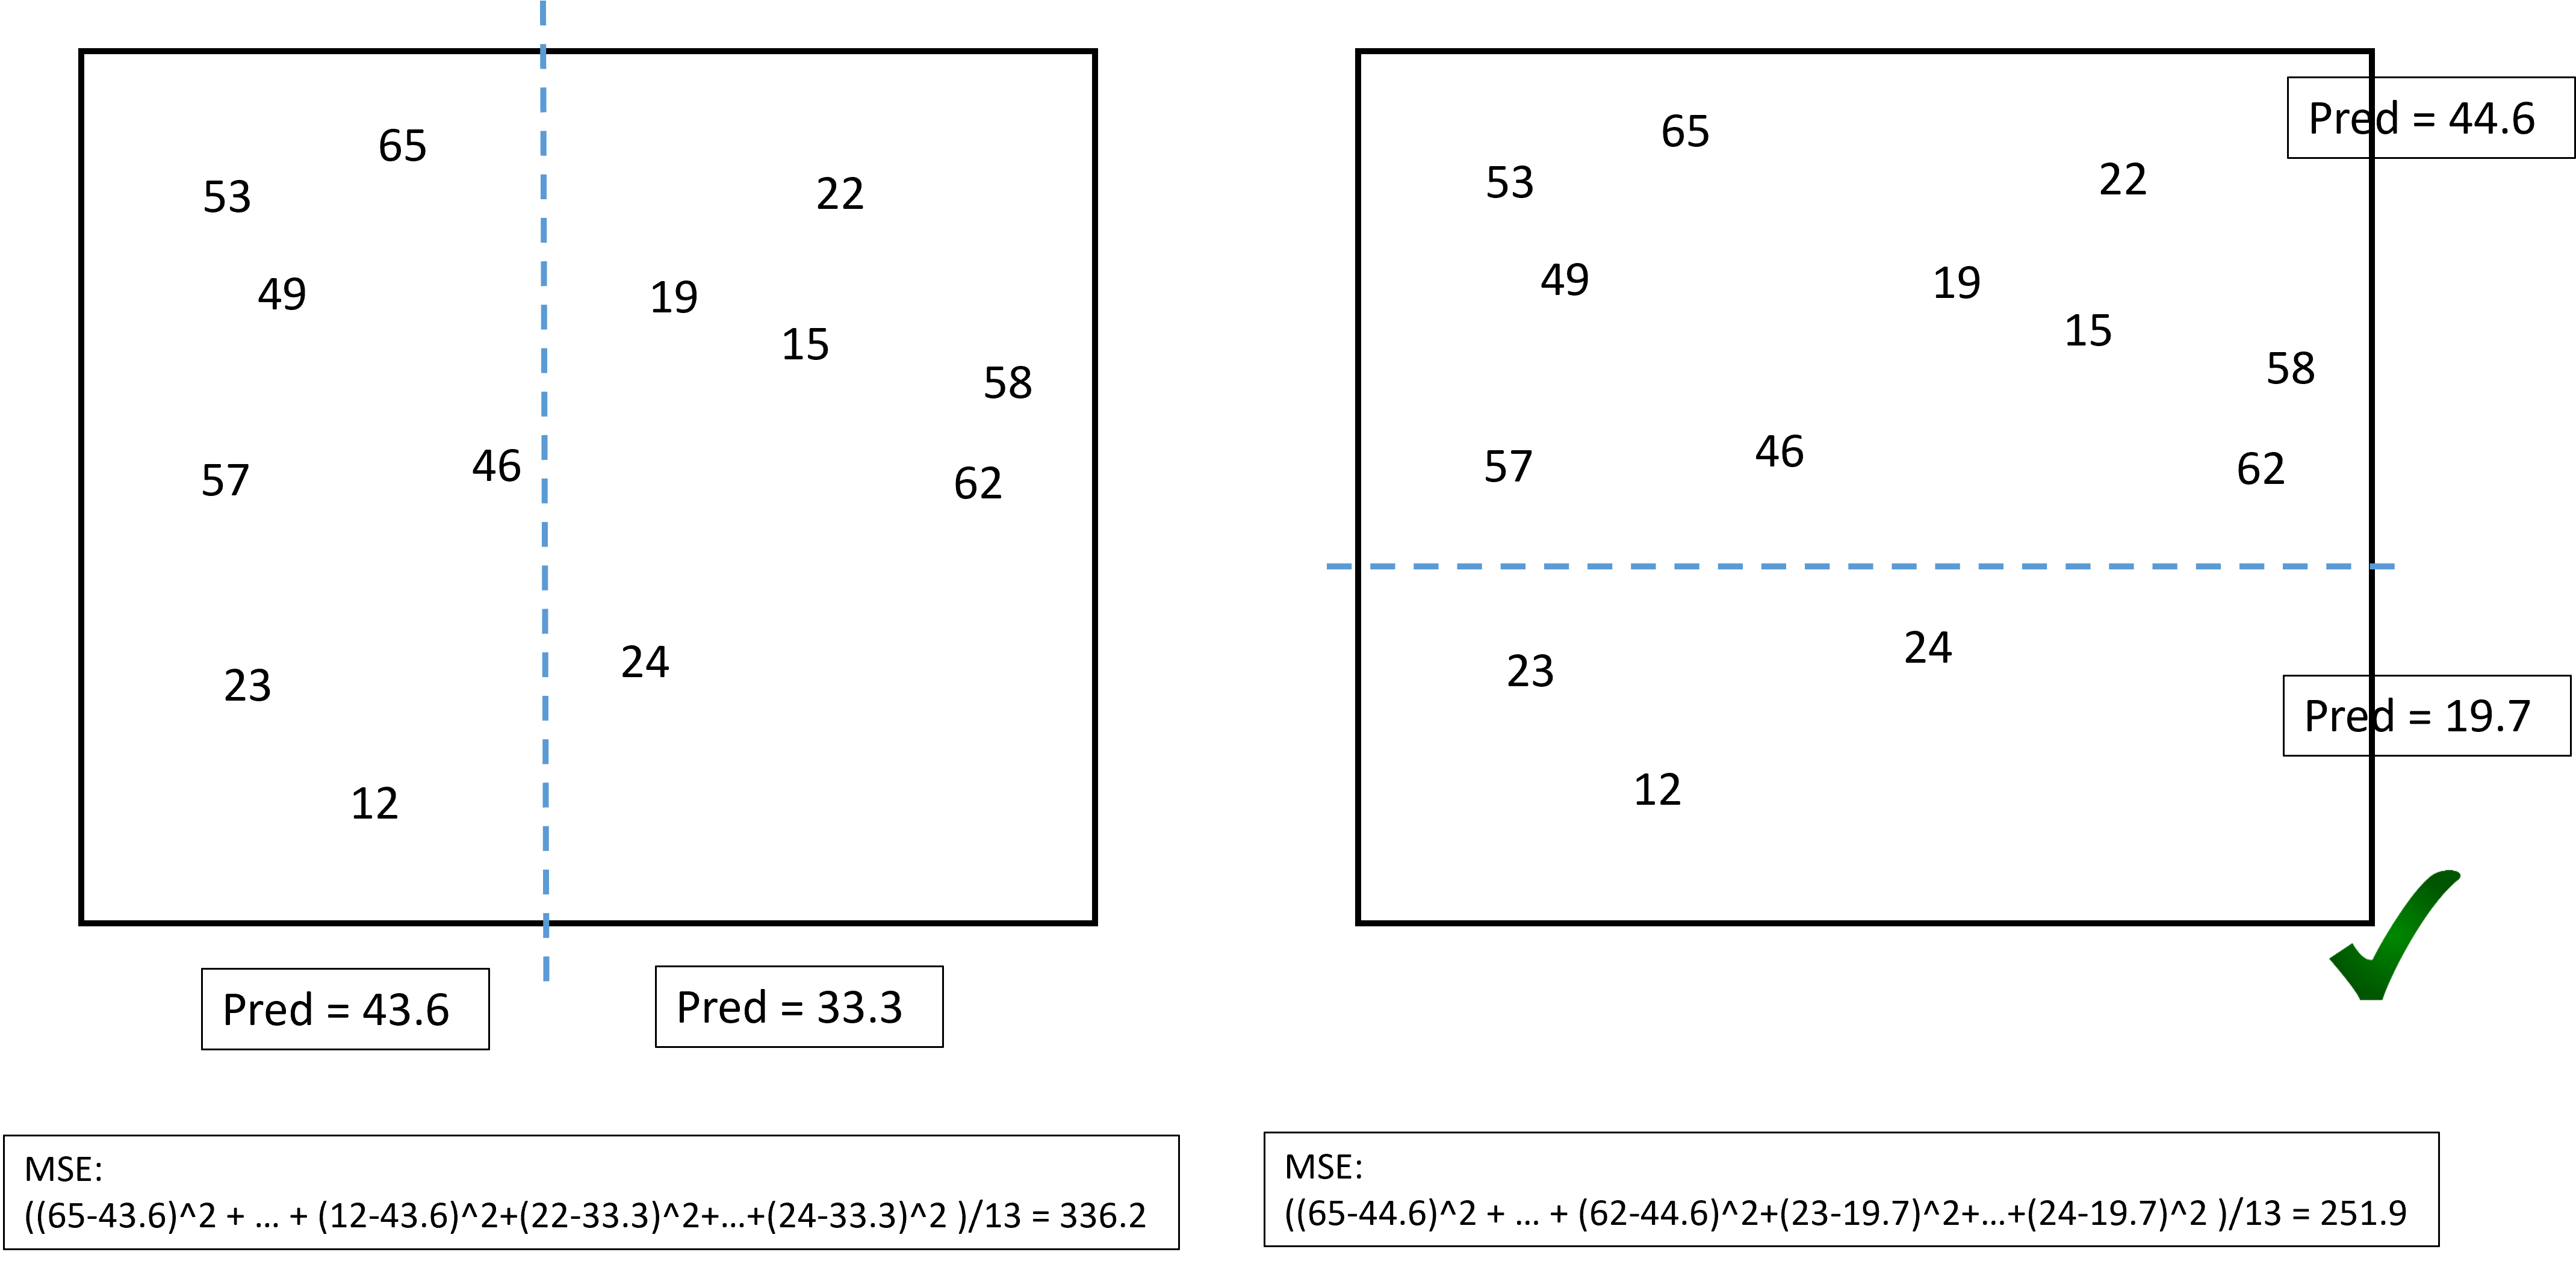
\includegraphics[width=9cm]{../../Graphs/RT_Build.png}
\end{center}
\end{frame}
%%%%%%%%%%%%%%%%%%%%%%%%%%%%%
\begin{frame}
\frametitle{A greedy algorithm}
On the following step, the two splits are built from the previous one. The left one is the best. 
\begin{center}
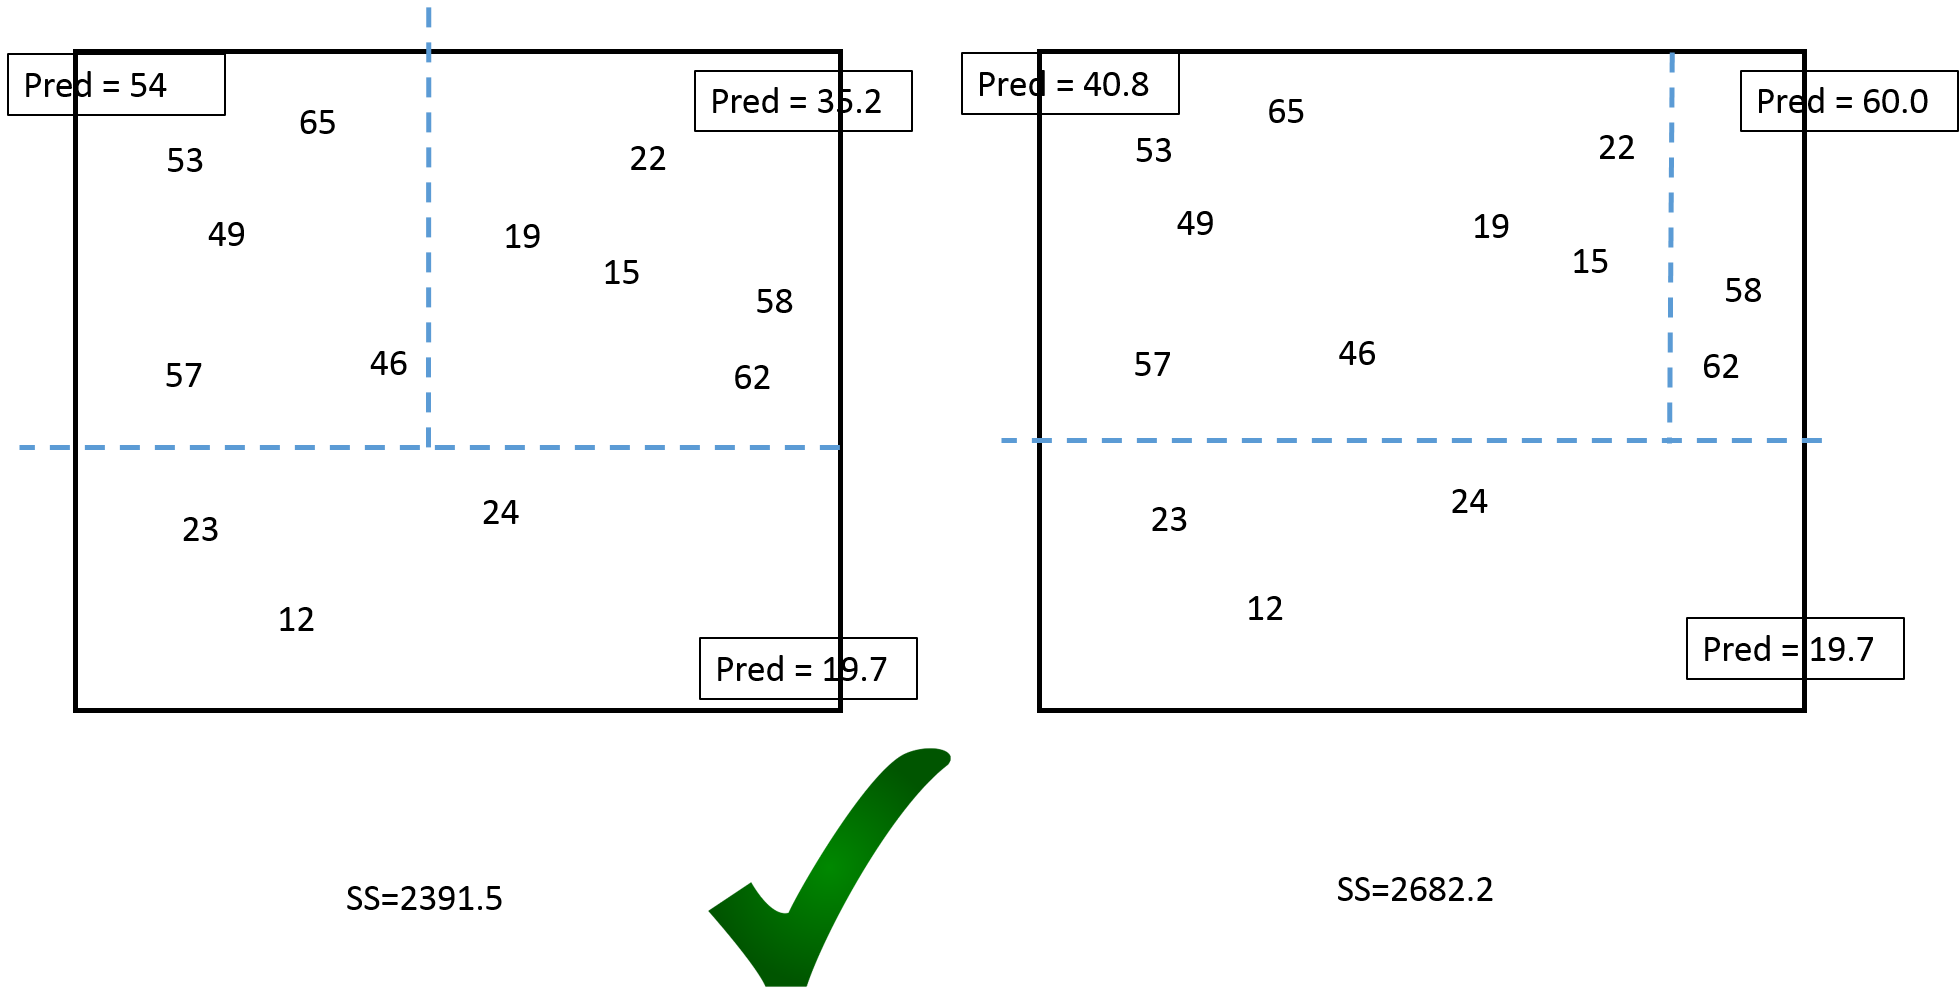
\includegraphics[width=9cm]{../../Graphs/RT_Build2.png}
\end{center}
The construction goes on like for the classification tree.  
\end{frame}
%%%%%%%%%%%%%%%%%%%%%%%%%%%%%
\begin{frame}
\frametitle{Impurity}
\begin{itemize}
\item A {\it good} split is define relative to a criterion of error called {\bf impurity} (measure of bad quality). 
\item A good split minimizes the impurity.
\item The impurity depends on the task: classification or regression.
\end{itemize}
\end{frame}
%%%%%%%%%%%%%%%%%%%%%%%%%%%%%
\begin{frame}
\frametitle{Impurity for classification}
Impurity $Q(D)$, for node $D$, with class prediction $c_D$. Common choices are
\begin{itemize}
\item {\bf Classification error}: 
$$
Q(D)=1-p_{c_D}(D).
$$
\item {\bf Gini index}:
$$
Q(D) = \sum_{c=1}^C p_c(D)\{1-p_c(D)\}.
$$
\item {\bf Entropy}:
$$
Q(D) = -\sum_{c=1}^C p_c(D)\log_2 p_c(D).
$$
\end{itemize}
\vspace{0.2cm} 
where, $p_c(D)$ is the proportion of instances with class $c$ in node a $D$
$$
p_c(D) = \frac{1}{|D|}\sum_{i\in D} 1_{\{y_i = c\}}.
$$
\end{frame}
%%%%%%%%%%%%%%%%%%%%%%%%%%%%%
\begin{frame}
\frametitle{Impurity: example}
Iris example: consider the final nodes from the left ($D_1$) to the right ($D_3$). Then
\begin{columns}
\begin{column}{0.5\textwidth}
\scriptsize
\begin{tabular}{|l|r|r|r|}
\hline
& $p_{\mbox{Set}}(D)$ & $p_{\mbox{Ver}}(D)$ & $p_{\mbox{Vir}}(D)$ \\
\hline
$D_1$ (Set) & $35/35$ & $0/35$ & $0/35$\\
\hline
$D_2$ (Ver) & $0/34$ & $33/34$ & $1/34$\\
\hline
$D_3$ (Vir) & $0/36$ & $2/36$ & $34/36$\\
\hline
\end{tabular}
\normalsize
\end{column}
\begin{column}{0.5\textwidth}
\begin{center}
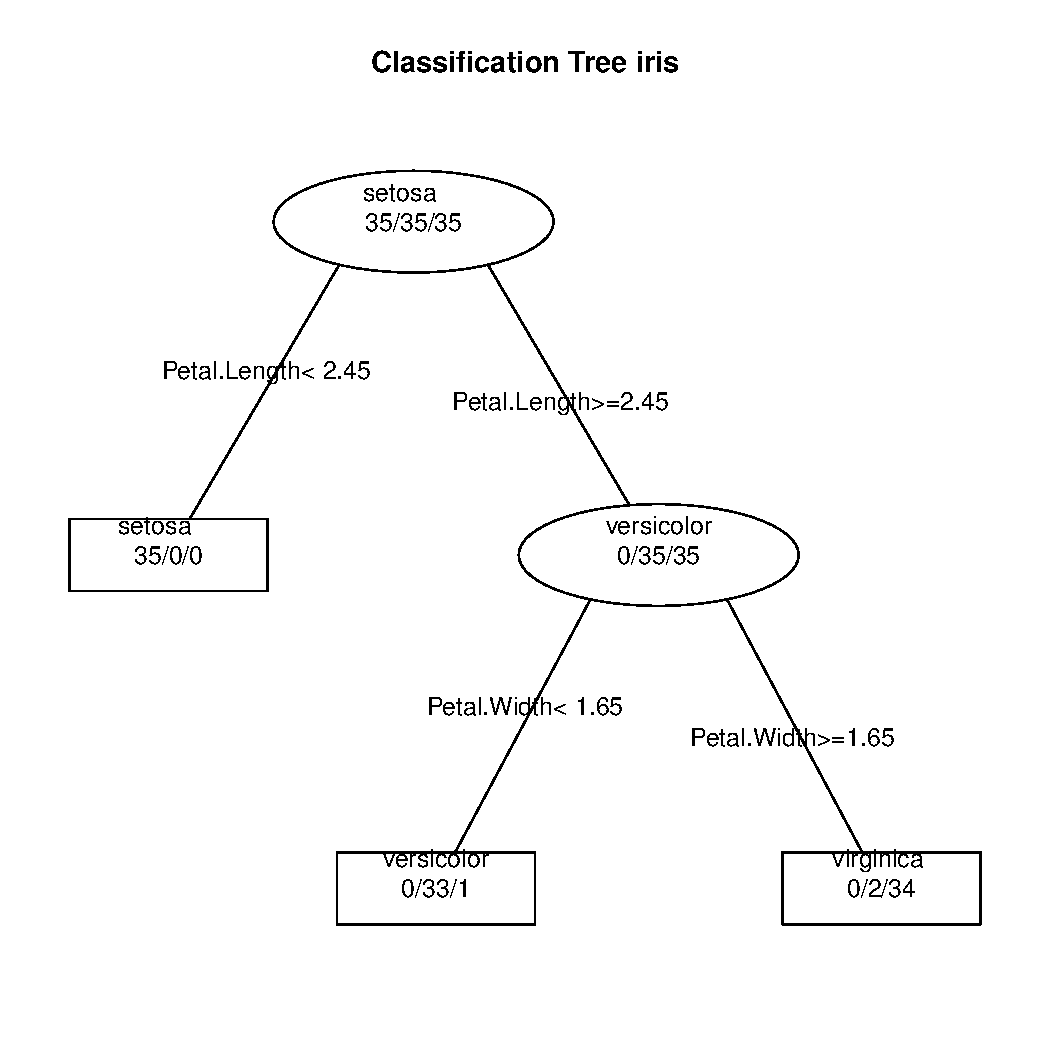
\includegraphics[width=5cm]{../../Graphs/IRIS_CART.pdf}
\end{center}
\end{column}
\end{columns}
\end{frame}
%%%%%%%%%%%%%%%%%%%%%%%%%%%%%
\begin{frame}
\frametitle{Impurity: example}
\begin{itemize}
\item Classification error for $D_3$:  
\begin{eqnarray*}
c(D_3)= \mbox{Vir}, \quad Q(D_3)= 1 - 34/36 = 1/18.\\
\end{eqnarray*}
\item Gini index for $D_3$:
\begin{eqnarray*}
Q(D_3)&=& \frac{0}{36}\times\left(1-\frac{36}{36}\right) + \frac{2}{36}\times\left(1-\frac{34}{36}\right) + \frac{34}{36}\times \left(1-\frac{2}{36}\right)\\
&=& \frac{0}{36}\times\frac{36}{36} + \frac{2}{36}\times\frac{34}{36} + \frac{34}{36}\times\frac{2}{36}\\
&=& 0.105\\
\end{eqnarray*}
\end{itemize}
\end{frame}
%%%%%%%%%%%%%%%%%%%%%%%%%%%%%
\begin{frame}
\frametitle{Impurity: example}
\begin{itemize}
\item Entropy for $D_3$:
\begin{eqnarray*}
Q(D_3)= -0\log_2(0)-\frac{2}{36}\log_2\frac{2}{36} - \frac{34}{36}\log_2\frac{34}{36}=0.31\\
\end{eqnarray*}
\end{itemize}
A "random" node with $(12/36, 12/36, 12/36)$ would have a Gini index of $0.67$ and an entropy of $1.58$. The lower the Gini index / entropy, the better the node.
\end{frame}
%%%%%%%%%%%%%%%%%%%%%%%%%%%%%
\begin{frame}
\frametitle{Impurity for regression}
In regression, most of the time, the impurity is the {\bf mean squared error} (MSE)
$$
Q(D) = \frac{1}{|D|} \sum_{i\in D}(y_i - c_D)^2.
$$
\end{frame}
%%%%%%%%%%%%%%%%%%%%%%%%%%%%%
\begin{frame}
\frametitle{Impurity}
Finally, for the whole tree ${\T}$ made of all the (final) nodes $D \in \T$, then the impurity of the tree is the total impurity of its nodes, weighted by their size:
$$
C(\T) = \sum_{D \in \T} |D| Q(D).
$$
A split is validated when it decreases the impurity of the tree.\\
\end{frame}
%%%%%%%%%%%%%%%%%%%%%%%%%%%%%
\begin{frame}
\frametitle{Stopping the growth}
The algorithm could go on splitting forever without stopping rules. Several rules can be used. For example in {\tt R} with {\tt rpart} (see {\tt ?rpart.control}):
\begin{itemize}
\item {\tt minsplit}: the minimum number of observations that must exist in a node in order for a split to be attempted (default is 20).
\item {\tt cp}: Any split that does not decrease the overall lack of fit by a factor of cp is not attempted (default to 0.1).
\item {\tt minbucket}: the minimum number of observations in any terminal node (default to {\tt minsplit/3}).  
\item etc.
\end{itemize}
Even with these rules, once the tree is grown, it might be too large. The procedure of cutting nodes is called {\tt pruning} the tree.  
\end{frame}
%%%%%%%%%%%%%%%%%%%%%%%%%%%%%%%%%%%%%%%%%%%%%
\section{Pruning the tree}
%%%%%%%%%%%%%%%%%%%%%%%%%%%%%%%%%%%%%%%%%%%%%
\begin{frame}
\frametitle{Occam's razor}
To prune the tree consists of simplifying it by cutting "useless" branches. It means that branches can be cut if they do not participate enough to the prediction quality. This is the same idea as the model selection: 
\begin{center}
Between two equally good models (in terms of predictions), choose the simplest one\footnote{Occam's razor}.
\end{center}
The idea is to control if the larger prediction quality of a long tree worth the extra complexity over a shorter tree (that is less precise). 
\end{frame}
%%%%%%%%%%%%%%%%%%%%%%%%%%%%%
\begin{frame}
\frametitle{Pruning concept}
There exist several ways to prune the tree. One of the most used is the {\bf 1-SE} rule. 
\begin{itemize}
\item Build a long tree (using the default stopping rules)
\item For all the sub-trees compute the error of the tree 
\item For the best tree (lowest error) compute the uncertainty on that error measure: the {\bf standard error} SE.
\item Any tree whose error is below the lowest error plus one SE is considered equivalent to the best tree.
\item Select the shortest tree among the equivalent to the best one.
\end{itemize}
\end{frame}
%%%%%%%%%%%%%%%%%%%%%%%%%%%%%
\begin{frame}
\frametitle{Pruning}
Example {\tt BreastCancer} data set (in {\tt mlbench}).\\
\scriptsize
The objective is to identify each of a number of benign or malignant classes. [...] Each variable except for the first was converted into 11 primitive numerical attributes with values ranging from 0 through 10. 
\normalsize
\begin{center}
\includegraphics[width=6cm]{../../Graphs/BreastCancerLongTree.pdf}
\end{center}
\end{frame}
%%%%%%%%%%%%%%%%%%%%%%%%%%%%%
\begin{frame}
\frametitle{Pruning}
Below, a measure of errors of all the sub-trees and the 1-SE limit from the best tree (size=4). The simplest equivalent to the best tree is of size 3.
\begin{center}
\includegraphics[width=7cm]{../../Graphs/BreastCancer_CPs.pdf}
\end{center}
\end{frame}
%%%%%%%%%%%%%%%%%%%%%%%%%%%%%
\begin{frame}
\frametitle{Pruning}
After the pruning, we will use the tree of size 3.
\begin{center}
\includegraphics[width=7cm]{../../Graphs/BreastCancerShortTree.pdf}
\end{center}
\end{frame}
%%%%%%%%%%%%%%%%%%%%%%%%%%%%%
\begin{frame}
\frametitle{Pruning details}
Technical details
\begin{itemize}
\item The error measure shown on the graph is relative.
\item The SE is computed using cross-validation (see later).
\item The 1-SE rule can be replaced by other rules (like cutting at a given CP, etc.). 
\end{itemize}
In practice, 
\begin{itemize}
\item the pruning is not a guarantee to obtain a good model. 
\item It should be used to simplify the model and avoid overfitting.
\item (empirical) it works well to build a very large tree then to prune it.
\end{itemize}
\end{frame}
%%%%%%%%%%%%%%%%%%%%%%%%%%%%%
\section{Surrogate splits}
%%%%%%%%%%%%%%%%%%%%%%%%%%%%%
\begin{frame}[fragile]
\frametitle{Surrogate splits and missing data}
An interesting property of the trees is that they can handle missing data to some extent. \\
\vspace{0.3cm}
When a split is made, several other splits were tried. The best ones not using the same feature are kept in memory and used in case.
\end{frame}
%%%%%%%%%%%%%%%%%%%%%%%%%%%%%
\begin{frame}[fragile]
\frametitle{Surrogate splits and missing data}
In {\tt R} the tree can be summarized by using function {\tt summary}. A partial output is\\
\tiny
\begin{verbatim}
Node number 3: 70 observations,    complexity param=0.4571429
  predicted class=versicolor  expected loss=0.5  P(node) =0.6666667
    class counts:     0    35    35
   probabilities: 0.000 0.500 0.500 
  left son=6 (34 obs) right son=7 (36 obs)
  Primary splits:
      Petal.Width  < 1.65 to the left,  improve=29.281050, (0 missing)
      Petal.Length < 5.05 to the left,  improve=26.250000, (0 missing)
      Sepal.Length < 6.15 to the left,  improve= 8.507149, (0 missing)
      Sepal.Width  < 2.95 to the left,  improve= 4.144737, (0 missing)
  Surrogate splits:
      Petal.Length < 4.75 to the left,  agree=0.929, adj=0.853, (0 split)
      Sepal.Length < 6.15 to the left,  agree=0.757, adj=0.500, (0 split)
      Sepal.Width  < 2.95 to the left,  agree=0.714, adj=0.412, (0 split)
\end{verbatim}
\normalsize
It describes node versicolor (0/35/35).
\end{frame}
%%%%%%%%%%%%%%%%%%%%%%%%%%%%%
\begin{frame}[fragile]
\frametitle{CART: surrogate splits and missing data}
\begin{itemize}
\item Primary split: "Petal.Width $<$ 1.65", the selected one. Improves the impurity by 29.28. The one below are its competitors. Not of direct use.
\item Surrogate splits: 
\begin{itemize}
\item "Petal.Length $<$ 4.75". If Petal.Width was messing, the prediction could be done using Petal.Length instead (go left on the tree). The agreement between the two rules is $92.9\%$ (measured on the training set). 
\item If Petal.Length is also missing, then "Sepal.Length $<$ 6.15" can be used. The agreement would be $75.5\%$.
\end{itemize}
\end{itemize}
\end{frame}
%%%%%%%%%%%%%%%%%%%%%%%%%%%%%
\section{Final words}
%%%%%%%%%%%%%%%%%%%%%%%%%%%%%
\begin{frame}
\frametitle{Final words}
CART looks great for
\begin{itemize}
\item Prediction (not a lazy learner).
\item Interpretation: the role and importance of each feature appears clearly on the tree.
\item Missing value: surrogate splits provide alternative rules.
\end{itemize}
However, 
\begin{itemize}
\item CART are {\it unstable}. 
\item Repeating the analysis on a similar data set (even very mildly different) can lead to very different trees. If the prediction performance will remain similar, the interpretation might be different.
\end{itemize}
\end{frame}
%%%%%%%%%%%%%%%%%%%%%%%%%%%%%
\end{document}

%%%%%%%%%%%%%%%%%%%%%%%%%%%%%
%%%%%%%%%%%%%%%%%%%%%%%%%%%%%
%%% Archives
%\begin{frame}
%\frametitle{Classification tree: representation of decision rules}
%Final classification (confusion matrix)
%\begin{center}
%\begin{tabular}{|c|c|c|c|}
%\hline
%& \multicolumn{3}{|c|}{Predicted}\\
%\hline
%Actual & Se & Ve & Vi\\
%\hline
%Se & 35 & 0 & 0\\
%\hline
%Ve & 0 & 33 & 1\\
%\hline
%Vi & 0 & 2 & 34\\
%\hline
%\end{tabular}
%\end{center}
%\end{frame}
%%%%%%%%%%%%%%%%%%%%%%%%%%%%%
%\begin{frame}
%\frametitle{CART: pruning}
%The graph is made of
%\begin{itemize}
%\item y-axis: quality of the tree prediction represented by a relative error (1=largest error; the empty tree).
%\item x-axis (top): tree complexity represented by the number of the nodes (size of the tree).
%\item x-axis (bottom): an overall quality-complexity indicator (see later).
%\end{itemize}
%We see that as the complexity increases, the error decreases less and less (fatigue effect or elbow). Increasing the tree becomes less and less interesting.
%\end{frame}
%%%%%%%%%%%%%%%%%%%%%%%%%%%%%%
%\begin{frame}
%\frametitle{CART: pruning}
%In addition, the uncertainty (standard error) on the relative error is computed for the "best" tree: horizontal dotted line.\\
%\vspace{0.3cm}
%The trees that are {\bf below} this dotted line are indistinguishable of the best tree. It is useless to have more complex trees.\\
%\vspace{0.3cm}
%This makes the 1-SE rule: choose the simplest tree among those below the dotted line.
%\end{frame}
%%%%%%%%%%%%%%%%%%%%%%%%%%%%%%
%\begin{frame}[fragile]
%\frametitle{CART: pruning}
%Example: with {\tt R} and its library {\tt rpart}, we can extract the following table\\
%\tiny
%\begin{verbatim}
%Classification tree:
%rpart(formula = class ~ mcv + gvh + lip + chg + aac + alm1 + 
    %alm2, data = ecoli.df)
%
%Variables actually used in tree construction:
%[1] aac  alm1 gvh  mcv 
%
%Root node error: 193/336 = 0.5744
%
%n= 336 
%
        %CP nsplit rel error  xerror     xstd
%1 0.388601      0   1.00000 1.00000 0.046959
%2 0.207254      1   0.61140 0.61658 0.045423
%3 0.062176      2   0.40415 0.46114 0.041910
%4 0.051813      3   0.34197 0.40415 0.040099
%5 0.031088      4   0.29016 0.38342 0.039359
%6 0.015544      5   0.25907 0.34715 0.037948
%7 0.010000      6   0.24352 0.34715 0.037948
%\end{verbatim}
%\normalsize
%The lowest error tree ($\T_m$) has an error of 0.34715, its standard deviation is 0.037948, that is, all the tree with xerror smaller than $0.34715+0.037948=0.385098$ are equivalent to $\T_m$.
%\end{frame}
%%%%%%%%%%%%%%%%%%%%%%%%%%%%%%
%\begin{frame}
%\frametitle{CART: pruning}
%Warning: coders of the package {\tt rpart} are probably not your friends...
%\begin{itemize}
%\item x-axis (top) on the plot is the {\bf size of the tree} whereas in the table it is the {\bf number of splits} (size = nsplit+1).
%\item y-axis on the plot is the {\bf relative} and the standard error is given for this relative error. In the table, the xstd is the standard error of the {\bf absolute} error. We don't have the std for the relative error.
%\end{itemize} 
%Of course, the final results are coherent and, in the example, the pruned tree will be of size 5 (i.e. 4 splits).
%\end{frame}
%%%%%%%%%%%%%%%%%%%%%%%%%%%%%%
%\begin{frame}
%\frametitle{CART: $k$-fold Cross-Validation}
%How is the standard deviation computed? Using cross-validation (CV).\\
%\vspace{0.2cm}
%The idea is 
%\begin{enumerate}
%\item Split the data set into $k$ several similar subsets (generally $k=10$ for CART), 
%\item Fit a tree of a given size $d$ on each of these subset,
%\item Compute the $k$ errors on each of these $k$ trees,
%\item Compute the mean and the standard deviation of these $k$ errors.
%\end{enumerate}
%Repeat this sequence for each size $d$. The results are given in columns {\tt xerror} and {\tt xstd}, and can be used for pruning.
%\end{frame}
%%%%%%%%%%%%%%%%%%%%%%%%%%%%%%
%\begin{frame}
%\frametitle{CART: $k$-fold Cross-Validation}
%About the usage of {\tt R} and package {\tt rpart}:
%\begin{itemize}
%\item when the function is used {\tt rpart}\footnote{cf exercises}, the CV is performed. There is a randomness here. If you repeat the fit, you will thus have different results. Use {\tt set.seed} to guarantee reproducibility.
%\item To make the pruning, use the function {\tt prune}. It requires the argument {\tt CP}. This can be found in the table, for the corresponding model\footnote{why not an argument {\tt nsplit}, I mean, WHY!?????}. Note that CP stands for complexity parameter, whose definition is quite technical and will be skipped for now.
%\end{itemize}
%\end{frame}
%%%%%%%%%%%%%%%%%%%%%%%%%%%%%%
%\begin{frame}[fragile]
%\frametitle{CART: pruning}
%{\bf Example}: with iris data.
%\begin{columns}[T]
%\begin{column}{0.5\textwidth}
%\tiny
%\begin{verbatim}
%Classification tree:
%rpart(formula = Species ~ ., data = iris[Train, ], method = "class")
%
%Variables actually used in tree construction:
%[1] Petal.Length Petal.Width 
%
%Root node error: 70/105 = 0.66667
%
%n= 105 
%
       %CP nsplit rel error   xerror     xstd
%1 0.50000      0  1.000000 1.185714 0.059574
%2 0.45714      1  0.500000 0.742857 0.073189
%3 0.01000      2  0.042857 0.085714 0.033978
%\end{verbatim}
%\normalsize
%\end{column}
%\begin{column}{0.5\textwidth}
%\vspace{1.5cm}
%\includegraphics[width=5cm]{../../Graphs/IRIS_CART_CP.pdf}
%\end{column}
%\end{columns}
%\end{frame}
%%%%%%%%%%%%%%%%%%%%%%%%%%%%%%
%\begin{frame}
%\frametitle{Concept}
%{\bf Example}: A regression tree was trained on the Facebook data taking the log of {\tt Lifetime.Post.Consumers} as the outcome.
%\begin{center}
%\includegraphics[width=10cm]{../../Graphs/FB_RT.png}
%\end{center}
%\end{frame}
%%%%%%%%%%%%%%%%%%%%%%%%%%%%%%
%\begin{frame}
%\frametitle{Prediction}
%{\bf Example}: for instance $i=1$
%\scriptsize
%\begin{center}
%\begin{tabular}{|c|c|}
%\hline
%{\tt log(Lifetime.Post.Consumers)} & 4.7\\
%{\tt Page.total.likes} & 139441 \\
%{\tt Type} & {\tt Photo}\\
%{\tt Category} & {\tt C2} \\
%{\tt Post.Month} & {\tt Dec} \\
%{\tt Post.Weekday} & {\tt Thu}\\
%{\tt Post.Hour} & 3\\
%{\tt Paid} & {\tt No}\\ 
%\hline
%\end{tabular} 
%\end{center}
%\normalsize
%The prediction is 5.5.
%\end{frame}
%%%%%%%%%%%%%%%%%%%%%%%%%%%%%%
%\begin{frame}
%\frametitle{Estimation}
%A tree $\T$ is estimated by minimizing the sum of squares of the errors
%$$
%SS_{\T} = \sum_{i=1}^n \left\{y_i - y(x_i)\right\}^2.
%$$
%The minimization is a very complex problem. In general a greedy algorithm is applied.\\ 
%\vspace{0.2cm}
%First note that, given a assignment of instances to nodes, the best estimate of $c_D$ is simply the average of the $y_i$'s assigned to $D$:
%$$
%c_D = \frac{1}{|D|}\sum_{i \in D} y_i.
%$$
%{\bf Example}: For the leftmost node, $421.1$ is the average of the outcomes of the instances assigned to this node.
%\end{frame}
%%%%%%%%%%%%%%%%%%%%%%%%%%%%%%
%\begin{frame}
%\frametitle{Estimation: a greedy algorithm}
%Again, similarly to classification tree, the tree is grown by looking at the best splitting feature $j$ and the best split point $s_j$.\\
%\vspace{0.2cm}
%Start: The tree has only one node $D_0$ and all instances are in it. 
%\begin{enumerate}
%\item Try feature $1$: the node $D_0$ is split into $D_1$ and $D_2$ along feature 1 looking for the best splitting point $s_1$, that is $D_1=\{i\, :\, x_{i1} < s_1\}$ and $D_2=\{i\, :\, x_{i1} \geq s_1\}$. To find $s_1$, solve
%$$
%\min_{s_1} \left[\sum_{i\in D_1}(y_i - c_1)^2 + \sum_{i\in D_2}(y_i - c_2)^2\right].
%$$
%\item Repeat step 2 for each feature $j$: the node $D_0$ is split into two nodes with the best $s_j$. 
%\item Keep the feature $j$: maximize the sum of squares reduction (i.e. best improvement).
%\item Assign the instances according to the split.
%\end{enumerate}
%\end{frame}
%%%%%%%%%%%%%%%%%%%%%%%%%%%%%%
%\begin{frame}
%\frametitle{Estimation: a greedy algorithm}
%Grow the tree: from a tree with nodes $D_1, \ldots, D_m$, 
%\begin{itemize}
%\item Scan each node, with each feature: select the best split $s$ each time
%\item Select the best feature for each node, and finally the best node.
%\item The best means the highest reduction in sum of squares.
%\end{itemize}
%This is repeated again and again until no improvement can be found or some stopping criteria are met (see the classification trees). 
%\end{frame}
%%%%%%%%%%%%%%%%%%%%%%%%%%%%%%
%\begin{frame}
%\frametitle{Impurity}
%The impurity measure of a node is the sum of squares
%$$
%Q(D) = \frac{1}{|D|} \sum_{i\in D}(y_i - c_D)^2.
%$$
%The cost criterion of the tree $\T$ is the sum of the impurities of all the nodes $D$ weighted by its size $|D|$
%$$
%C(\T) = \sum_{D\in \T} |D| Q(D)
%$$
%\end{frame}
%%%%%%%%%%%%%%%%%%%%%%%%%%%%%%
%\begin{frame}
%\frametitle{Example}
%Suppose that we have two features and a numerical outcome $y$ as shown below. In each area, the prediction is the average of all the observations. The right split is better than the left one because the sum of the squares is lower.
%\begin{center}
%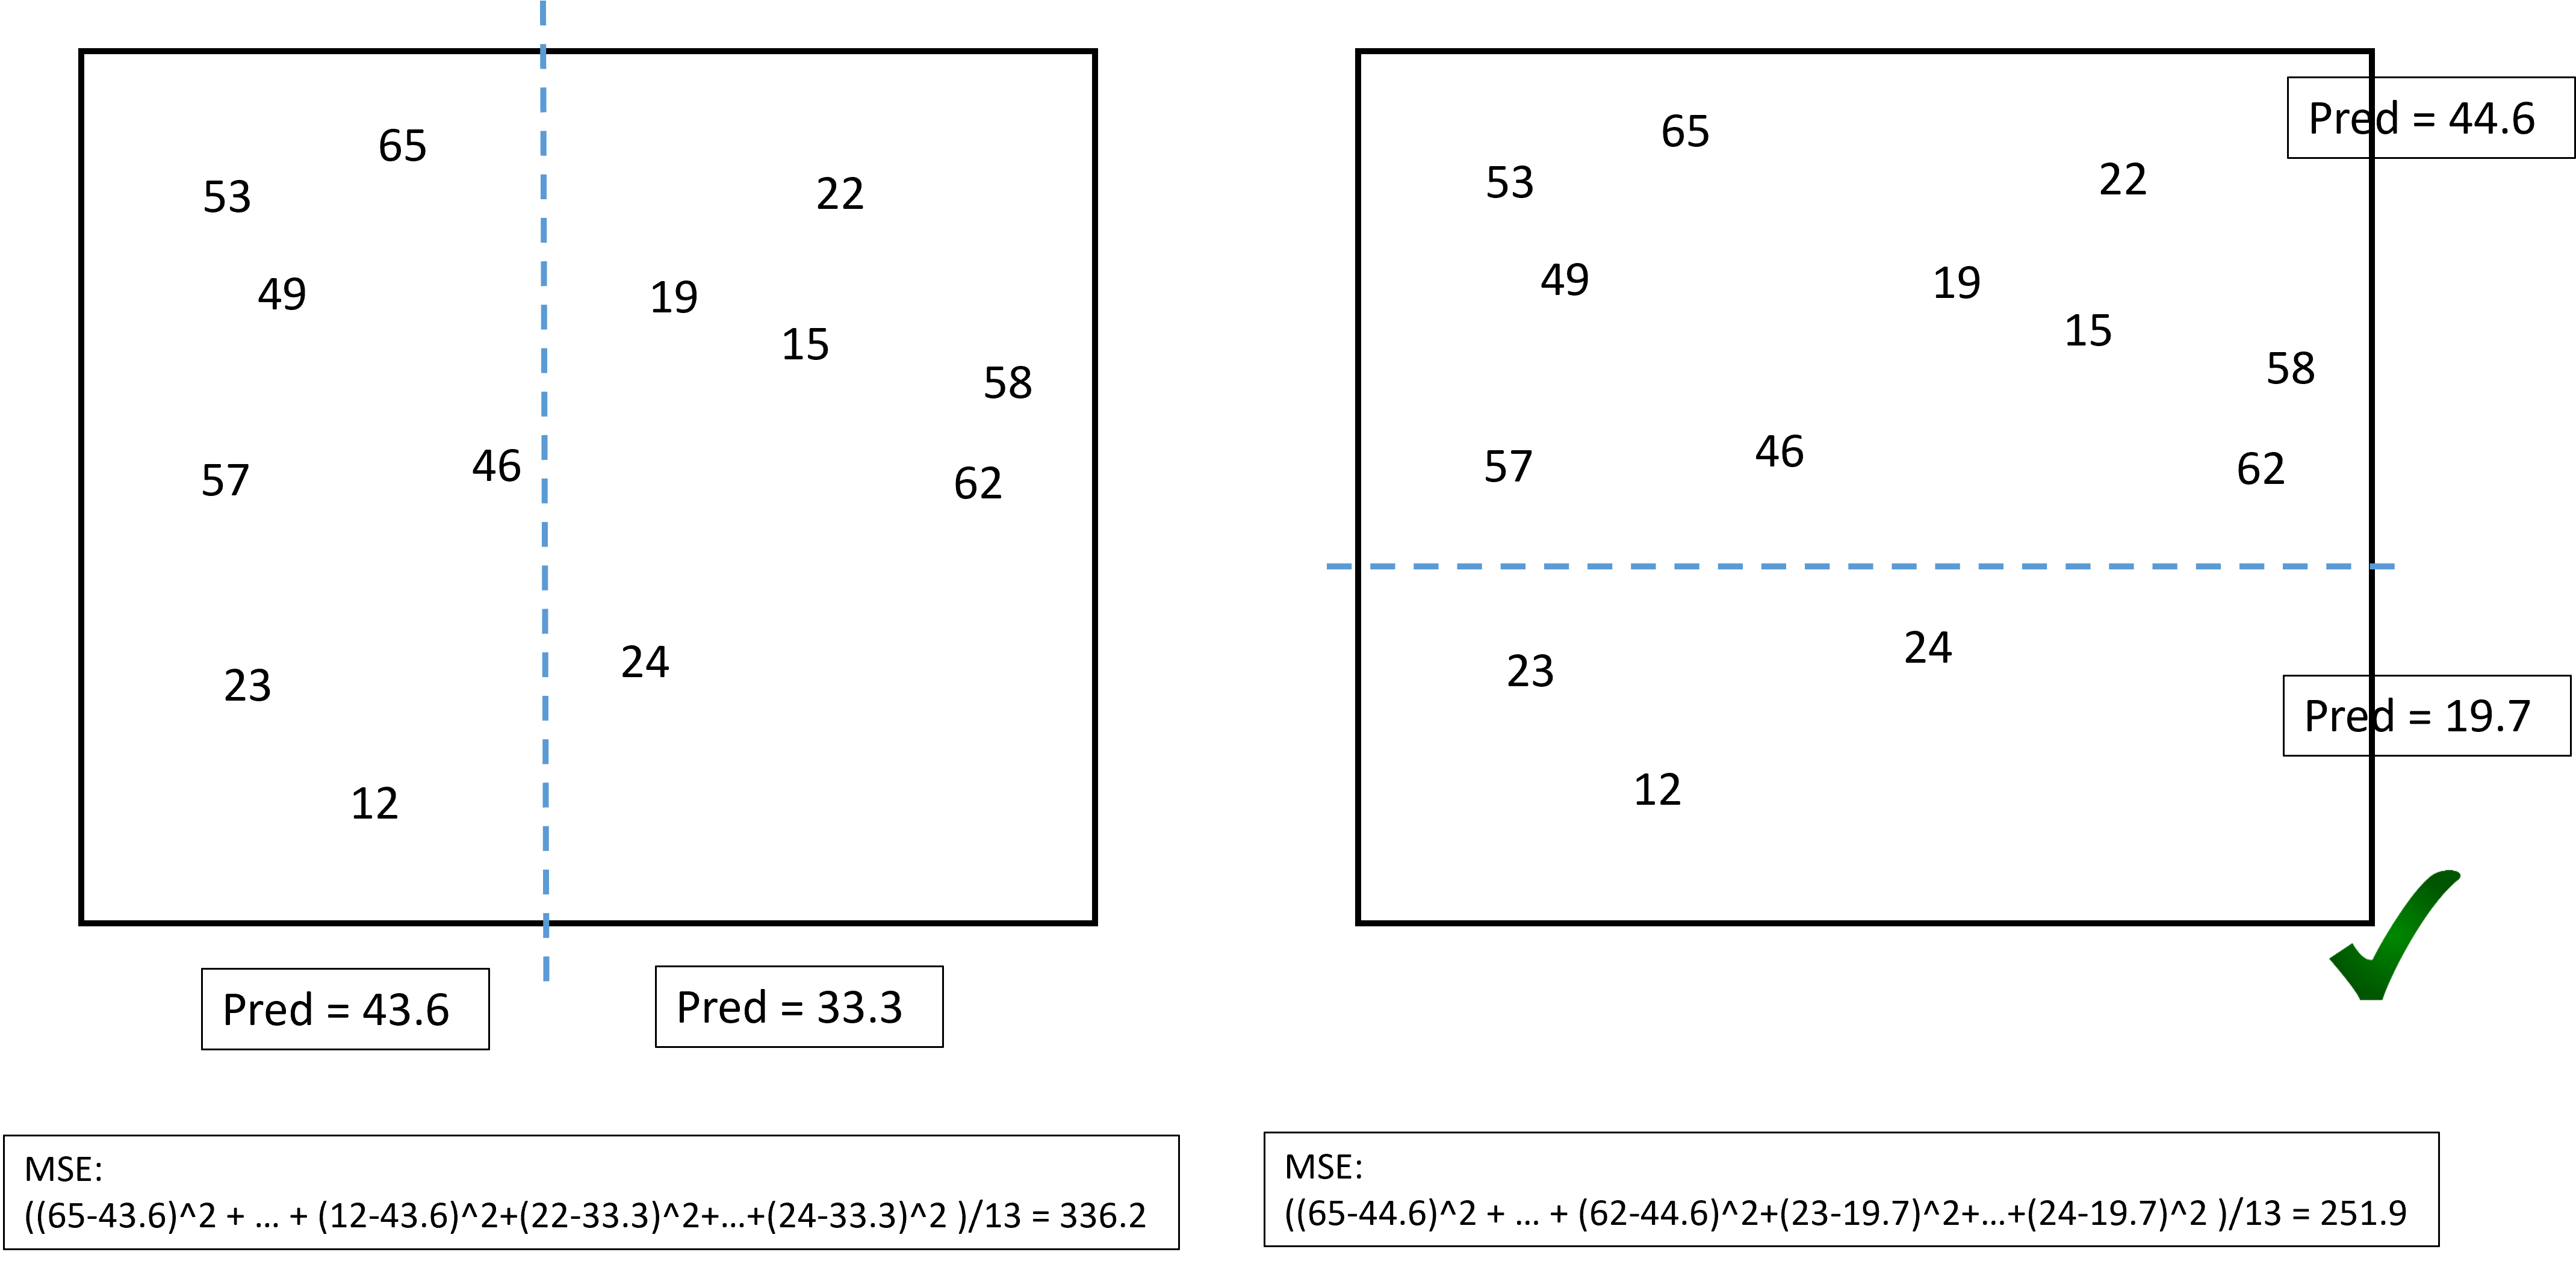
\includegraphics[width=9cm]{../../Graphs/RT_Build.png}
%\end{center}
%\end{frame}
%%%%%%%%%%%%%%%%%%%%%%%%%%%%%%
%\begin{frame}
%\frametitle{Example}
%On the following step, the two splits are built from the previous one. The left one is the best. 
%\begin{center}
%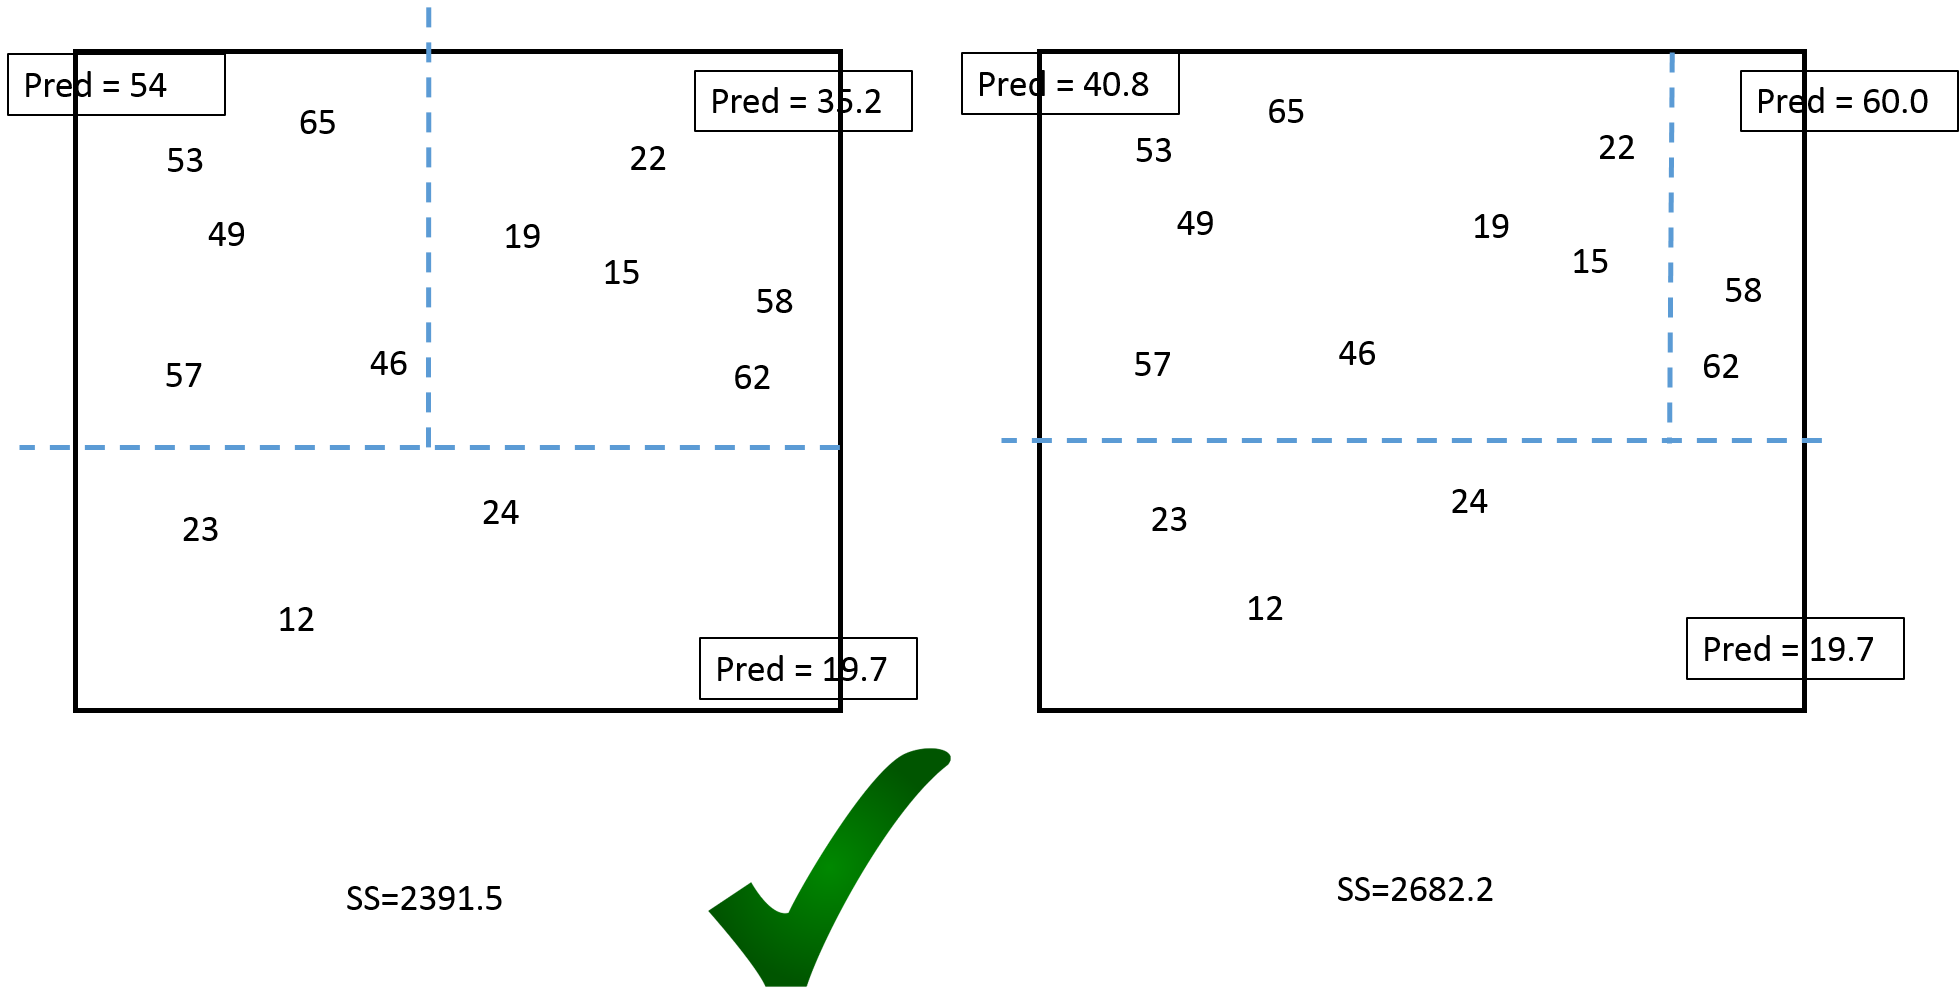
\includegraphics[width=9cm]{../../Graphs/RT_Build2.png}
%\end{center}
%The construction goes on like for the classification tree.  
%\end{frame}
%%%%%%%%%%%%%%%%%%%%%%%%%%%%%%
%\begin{frame}[fragile]
%\frametitle{Pruning}
%The pruning is based on the same principles and done the same way as for classification trees. A cross validation is applied to estimate an error measure on the tree and its standard deviation.\\
%\vspace{0.2cm}
%{\bf Example}: With the Facebook data set.\\
%\tiny
%\begin{verbatim}
%> printcp(fb1.rt)
%
%Regression tree:
%rpart(formula = log(Lifetime.Post.Consumers) ~ Page.total.likes + 
    %Type + Category + Post.Month + Post.Weekday + Post.Hour + 
    %Paid, data = facebook.dat)
%
%[...]
         %CP nsplit rel error  xerror     xstd
%1  0.125541      0   1.00000 1.00242 0.088916
%2  0.122109      1   0.87446 0.88533 0.091837
%3  0.052674      2   0.75235 0.76489 0.084913
%4  0.042871      3   0.69968 0.76317 0.085686
%5  0.033342      4   0.65681 0.73721 0.085579
%6  0.019146      5   0.62346 0.71597 0.082959
%7  0.016526      6   0.60432 0.72877 0.082121
%8  0.013644      7   0.58779 0.75138 0.085962
%9  0.012505      8   0.57415 0.74602 0.086357
%10 0.010000     10   0.54914 0.75042 0.087218
%\end{verbatim}
%\normalsize
%\end{frame}
%%%%%%%%%%%%%%%%%%%%%%%%%%%%%%
%\begin{frame}
%\frametitle{Pruning}
%Lowest {\tt xerror} is 0.71597 with an uncertainty of {\tt xstd} 0.082959. With the 1-SE rule, it is indistinguishable from a tree with {\tt xerror} of 
%$$
%0.71597 + 0.082959 = 0.798929
%$$
%In our search for a simpler tree, it is thus equivalent to tree with 2 splits, i.e. 3 nodes. This can be seen at once with the {\tt plotcp} function:
%\begin{center}
%\includegraphics[width=5cm]{../../Graphs/FB_CP.png}
%\end{center}
%\end{frame}
%%%%%%%%%%%%%%%%%%%%%%%%%%%%%%
%\begin{frame}[fragile]
%\frametitle{Pruning}
%\scriptsize
%\begin{verbatim}
%fb2.rt <- prune(fb1.rt, cp=0.052674)
%\end{verbatim}
%\begin{center}
%\includegraphics[width=8cm]{../../Graphs/FB_RT_pruned.png}
%\end{center}
%\end{frame}
%%%%%%%%%%%%%%%%%%%%%%%%%%%%%%
%\begin{frame}
%\frametitle{Predictions}
%The predictions of a RT are constant within each nodes. Small trees can provide ``unrealistic'' prediction pictures. Only a model score can provide a clear judgment on the model quality.\\
%\scriptsize
%\begin{center}
%\includegraphics[width=5cm]{../../Graphs/FB_Pred_log.png}
%\includegraphics[width=5cm]{../../Graphs/FB_Pred.png}
%\end{center}
%\end{frame}
%%%%%%%%%%%%%%%%%%%%%%%%%%%%%%
%\begin{frame}
%\frametitle{Concept}
%Regression trees are similar to classification trees.\\ 
%\vspace{0.2cm}
%A value $c_D$ is assigned to each node $D$. The prediction function can be written as
%$$
%y(x) = \sum_{D \in \T} c_D \delta_D(x),
%$$ 
%where the sum above is over $D$, the nodes of the tree $\T$, and
%$$
%\delta_D(x) =\left\{
%\begin{array}{ll}
%1,& \mbox{if } x\in D,\\
%0,& \mbox{if } x\notin D,
%\end{array}
%\right.
%$$
%In short, an instance is assigned to a node $D$ according to its features. The prediction of the outcome is the value $c_D$ of the node $D$.
%\end{frame}
%%%%%%%%%%%%%%%%%%%%%%%%%%%%%%
